\documentclass{llncs}[11pt]

\def\isanonymous{0}
\def\isshort{0}

\usepackage{ifthen}
\newcommand{\anonymous}[2]{
\ifthenelse{\equal{\isanonymous}{1}}
{{#1}}
{{#2}}
}

\newcommand{\submission}[2]{\ifthenelse{\equal{\isshort}{1}}{{#1}\xspace}{{#2}\xspace}}


\ifthenelse{\equal{\isshort}{0}}{
\usepackage{a4wide}
}{}

\usepackage[utf8x]{inputenc}
\usepackage{amsmath,amsfonts,amssymb}
\usepackage{xspace}
\usepackage{tikz,pgfplots}

%%%%%%%%%%%%%%%%%%%%%%%%%%%%%%%%%%%%%%%%%%%%%%%%%%%%%%%%%%%%%%%%
% Speed up compilation by caching Tikz picktures
%
% when you change a tikz picture run: 
%
%  pdflatex -shell-escape bkw-small-secret
%
% You can also simply comment out the two lines below to go back 
% to the normal behaviour
%%%%%%%%%%%%%%%%%%%%%%%%%%%%%%%%%%%%%%%%%%%%%%%%%%%%%%%%%%%%%%%%

%\usetikzlibrary{external}
%\tikzexternalize[prefix=figures/] % activate!

\usepackage{embedfile}

\usepackage{url}
\usepackage[vlined,linesnumbered]{algorithm2e}

\usepackage[index,multiuser]{fixme}
\fxsetup{
    status=draft,
    layout=pdfcnote,
    theme=color
}

\FXRegisterAuthor{malb}{amalb}{malb}
\FXRegisterAuthor{lp}{alp}{lp}
\FXRegisterAuthor{rf}{arf}{rf}

\newcommand\LWE{\ensuremath{{\rm LWE}}\xspace}
\newtheorem{assumption}{Assumption}

\newcommand{\tildeO}[1]{\ensuremath{\tilde{\mathcal{O}}(#1)}\xspace}

\newcommand{\heading}[1]{{\vspace{6pt}\noindent\sc{#1.}}}

\newcommand{\bigO}[1]{\ensuremath{\mathcal{O}\left(#1\right)}\xspace}
\newcommand{\poly}{ {\rm poly}(n)}
\newcommand{\chig}{\ensuremath{\chi_{\alpha,q}}}
\newcommand{\chis}{\ensuremath{\psi}}
\newcommand{\U}[1]{\ensuremath{\mathcal{U}(#1)\xspace}}
\newcommand{\Z}{\ensuremath{\mathbb{Z}}\xspace}
\newcommand{\Zq}{\ensuremath{\mathbb{Z}_q}\xspace}
\newcommand{\Zp}{\ensuremath{\mathbb{Z}_p}\xspace}
\newcommand{\Zqchi}{\ensuremath{\mathbb{Z}^{\Phi_{\zeta}}_q}[\vec{x}]\xspace}
\newcommand{\Ldis}{L_{\mathbf{s},\chi}\xspace}

\newcommand{\Bdis}[1]{B_{\mathbf{s},\chi}(b,#1,p)\xspace}
\newcommand{\Bdissm}[1]{B_{small,\mathbf{s},\chi}(b,#1,p)\xspace}
\newcommand{\sample}{\ensuremath{\leftarrow_{\$}}}

\newcommand{\CDF}[1]{\textnormal{CDF}\left(#1\right)\xspace}
\newcommand{\E}{\ensuremath{\textnormal{E}}}
\newcommand{\Var}{\ensuremath{\textnormal{Var}}}

\newcommand{\abs}[1]{\ensuremath{\left|#1\right|}\xspace}

\renewcommand{\vec}[1]{\mathbf{#1}\xspace}
\newcommand{\shortvec}[1]{\tilde{\mathbf{#1}}\xspace}
\newcommand{\mat}[1]{\ensuremath{\mathbf{#1}}\xspace}

\newcommand{\dotp}[2]{\ensuremath{\left\langle {#1},{#2}\right\rangle}\xspace}
\newcommand{\N}[1]{\ensuremath{\mathcal{N}({#1)}}}
\newcommand{\round}[1]{\ensuremath{\left\lfloor{#1}\right\rceil}\xspace}

\def\abn{\lceil n/b \rceil}


\title{Lazy Modulus Switching for the BKW Algorithm on LWE}
\anonymous{\author{} \institute{}}{
\author{Martin R.~Albrecht \inst{1} \and Jean-Charles Faugère \inst{3,2,4} \and Robert Fitzpatrick \inst{5} \and Ludovic Perret \inst{2,3,4}}
\institute{
Technical University of Denmark, Denmark \and
Sorbonne Universités, UPMC Univ Paris 06, POLSYS, UMR 7606, LIP6, F-75005, Paris, France \and
INRIA, Paris-Rocquencourt Center, POLSYS Project\and
CNRS, UMR 7606, LIP6, F-75005, Paris, France \and
Information Security Group\\
Royal Holloway, University of London\\
Egham, Surrey TW20 0EX, United Kingdom \\ 
\email{maroa@dtu.dk, jean-charles.faugere@inria.fr, robert.fitzpatrick.2010@live.rhul.ac.uk, ludovic.perret@lip6.fr}  
}}


\parindent 0em
\parskip 0.9em

\begin{document}

\maketitle

\begin{abstract}
Some recent constructions based on LWE do not sample the secret uniformly at random but rather from some distribution which produces small entries. The most prominent of these is the binary-LWE problem where the secret vector is sampled from $\{0,1\}^{\ast}$ or $\{-1,0,1\}^{\ast}$. We present a variant of the BKW algorithm for binary-LWE and other small secret variants and show that this variant reduces the complexity for solving binary-LWE. We also give estimates for the cost of solving binary-LWE instances in this setting and demonstrate the advantage of this BKW variant over  standard BKW and lattice reduction techniques applied to the SIS problem. Our variant can be seen as a combination of the BKW algorithm with a lazy variant of modulus switching which might be of independent interest.
\end{abstract}

\section{Introduction} \label{sec:intro}
Learning With Errors (\LWE) \cite{regev:acm09} has received  widespread attention from the cryptographic community since its introduction. \LWE-based cryptography is mainly motivated by its great flexibility for instantiating cryptographic solution as well as a deep worst-case/average-case connections \cite{regev:acm09}: solving \LWE{} on the average is not easier than solving worst-case instances of several famous lattice approximation problems.

The motivation behind this work comes from the observation that some recent constructions based on \LWE do not sample the secret uniformly at random but rather from some distribution which produces small entries (e.g.\ \cite{applebaum-cash-peikert-sahai:crypto2009,DBLP:conf/tcc/AkaviaGV09,DBLP:conf/innovations/GoldwasserKPV10,gentry-halevi-smart:crypto2012,DBLP:conf/tcc/Pietrzak12}). From a theoretical point of view, this is motivated by the observation that every \LWE instance can be transformed into an instance where the secret follows the same distribution as the noise \cite{applebaum-cash-peikert-sahai:crypto2009}.\footnote{also in \cite{kirchner:eprint2011} for the LPN case.} However, many constructions use secrets which are considerably smaller.
For example, binary-\LWE samples the secret from $\{0,1\}^*$ \cite{brakerski-langlois-peikert-regev-stehle:stoc13} or $\{-1,0,1\}^*$ \cite{gentry-halevi-smart:crypto2012}. The presence of such small secrets provokes the question of what implications such choices have on the security of \LWE. Is solving \LWE with, say, binary secrets easier than standard \LWE? From a theoretical point of view, \cite{brakerski-langlois-peikert-regev-stehle:stoc13} proves that their binary-\LWE is as secure as \LWE{}. In this paper, we try to address the question from an algorithmic point of view; i.e. what is the actual impact of small secrets on concrete parameters.    

\subsection{Algorithms for Solving \LWE}
Three families of algorithms for solving \LWE are known in the literature. The most prominent approach is to reduce \LWE to a problem that can be solved via lattice reduction, for example, by reducing it to the Short Integer Solution (SIS) problem. Indeed, most parameter choices in the literature are based on the hardness of lattice reduction such as \cite{LindnerP10,chen-nguyen:asiacrypt2011,liu-nguyen:ctrsa2013}. These estimates for a given set of parameters $n$ (number of components of the secret), $q$ (size of the modulus) and  $\sigma$ (standard deviation of the noise) are usually produced by extrapolating running times from small instances.

A second approach is due to Arora and Ge who reduce \LWE to solving a  system of non-linear equations \cite{arora-ge:icalp2011}. This algorithm allow us to solve \LWE in sub-exponential time as soon as the Gaussian distribution  is sufficiently narrow, i.e.\ $\alpha \cdot q <\sqrt{n}$. Recall that  the security reduction \cite{regev:acm09} for \LWE requires to consider discrete Gaussian  with standard deviation $\alpha \cdot q$ strictly bigger than $\sqrt{n}$.
However, from a practical point of view, the constants involved in this algorithm are so large that it is much more costly than other approaches for the parameters typically considered in cryptographic applications \cite{SCC12_AG}. 

The third family of algorithms are combinatorial algorithms which can all be seen as variants of the BKW algorithm. The BKW algorithm was proposed by Blum, Kalai and Wasserman~\cite{blum-kalai-wasserman:acm2003} as a method for solving the Learning Parity with Noise problem, with sub-exponential complexity, requiring $2^{\bigO{n / \log n}}$ samples, space and time. The algorithm can be adapted for tackling \LWE with complexity $2^{\bigO{n}}$ when the modulus is taken to be polynomial in $n$ \cite{regev:acm09}. BKW proceeds by splitting the $n$ components of LWE samples into $a$ groups of $b$ components each. For each of the $a$ groups of components the algorithm then searches for collisions in these $b$ components to eliminate them. The overall complexity of the algorithm is  $\approx \left(a^2n\right) \cdot \frac{q^b}{2}$ operations, and $a\cdot \frac{q^b}{2}$ memory, where $a$ and $b$ depend on the $n, q$ and $\alpha$.

The behaviour of the algorithm is relatively well understood and it was shown to outperform lattice reduction estimates when reducing LWE to SIS (when $q$ is small), thus it provides a solid basis for analysing the concrete hardness of LWE instances \cite{albrecht-cid-faugere-fitzpatrick-perret:dcc2013}.

\subsection{Organisation of the Paper and Main Results}
While none of the algorithms above take advantage of the presence of small secrets, we may combine them with  {\it modulus switching}. Recall that modulus switching was initially introduced to improve the performance of homomorphic encryption schemes \cite{brakerski-vaikuntanathan:focs2011} and was recently used to reduce the hardness of \LWE with polynomially sized moduli to GAPSVP \cite{brakerski-langlois-peikert-regev-stehle:stoc13}. Modulus switching is essentially the same as computing with a lower precision similar to performing floating point computations with a low fixed precision. Namely, let $\big(\vec{a},
c=\dotp{\vec{a}}{\vec{s}} + e\big) \in \Zq^n \times \Zq$ be \LWE sample 
where $\vec{s} \in \Zq^n$ is the secret vector, and $e \in \Zq$ is an error. Let also some $p < q $ and consider $\big(\round{{p}/{q} \cdot \vec{a}}, \round{{p}/{q} \cdot c}\big)$ with
\begin{small}
\begin{align}
\label{eq:roundingerror}
\round{\frac{p}{q} \cdot c} =& \round{\frac{p}{q} \big( \dotp{\vec{a}}{\vec{s}}+q \cdot u +e \big)}, \mbox{ for some $u \in \Z$}\nonumber\\
\round{\frac{p}{q} \cdot c} =& \round{ \dotp{ \frac{p}{q} \cdot \vec{a} }{\vec{s} }_{p} + \frac{p}{q} \cdot e} =  \round{ \dotp{ \round{ \frac{p}{q} \cdot \vec{a} }}{\vec{s} }_{p} + \dotp{\frac{p}{q} \cdot \vec{a} - \round{ \frac{p}{q} \cdot \vec{a} }}{\vec{s}}_{p} + \frac{p}{q} \cdot e}\nonumber\\
  =& \dotp{ \round{ \frac{p}{q} \cdot \vec{a} }}{\vec{s} }_{p} + \dotp{\frac{p}{q} \cdot \vec{a} - \round{ \frac{p}{q} \cdot \vec{a} }}{\vec{s}}_{p} + \frac{p}{q} \cdot e + e' \textnormal{, where } e' \in [-0.5,0.5] \nonumber\\
  =& \dotp{ \round{ \frac{p}{q} \cdot \vec{a} }}{\vec{s} }_{p} + e'' + \frac{p}{q}\cdot e + e'.
\end{align}
\end{small}
where $\dotp{\vec{x}}{\vec{y}}_{p}$ denotes the modulo $p$ inner product of $\vec{x}$ and $\vec{y}$.

Since ${p}/{q} \cdot \vec{a} - \round{ {p}/{q} \cdot \vec{a} }$ takes values $\in [-0.5,0.5]$ we have that $e''$ is small if $\vec{s}$ is small. We may hence compute with the smaller `precision' $p$ 
at the cost of a slight increase of the noise rate by  a `{\it rounding error}' $e''$. 
 
Modulus switching allows to map a \LWE{} instance $\bmod \, q$ to a scaled instance of \LWE{} $\bmod \, p$.
Thus, modulus switching can be used in the solving of small secret instances of \LWE, a folklore approach which has not been explicitly studied in the literature. Namely, if we pick $p$ such that $e''$ is not much larger than $p/q \cdot e$ then, for example, the running time of the BKW 
algorithm improves from $(a^2n)\cdot \frac{q^b}{2}$ to $(a^2n)\cdot \frac{p^b}{2}$. Since typically $b \approx n/\log n$ 
this may translate to substantial improvements. Indeed, we can pick $p$ such that $\abs{\dotp{{p}/{q} \cdot \vec{a} - 
\round{ {p}/{q} \cdot \vec{a} }}{\vec{s}}} \approx p/q \cdot \abs{e}$.
This implies ${\sigma_s}\cdot \sqrt{\frac{n}{12}} \approx p/q \cdot \sigma$, or
$
p \approx \min\left\{q, \frac{\sigma_s}{\sigma}\cdot \sqrt{\frac{n}{12}} \cdot q \right\}$, where $\sigma_s$ is the standard deviation of elements in the secret $\vec{s}$.

In this paper, we refine this approach and present a variant of the BKW algorithm which fuses modulus switching and BKW-style reduction. In particular, this work has two main contributions. Firstly, in Section~\ref{sec:bkw-algorithm} we present a modulus switching strategy for the BKW algorithm in which switching is delayed until necessary.  In a nutshell, recall that the BKW algorithm performs additions of elements which collide in certain components. Our variant will search for such collisions in `low precision' $\Zp$ but will perform arithmetic in `high precision' $\Zq$.  We call {\it rounding error} the inner product of the sub-vector of `low bits' of $\vec{a}$ with the secret $\vec{s}$. Our strategy permits to decrease rounding errors and allows to reduce $p$ by a factor of $\sqrt{a}$.

Secondly, this perspective enables us to choose reductors in the BKW algorithm which minimise the rounding errors further (Section \ref{sec:control-growth}). Namely, we favour components $a$ with small distance $\abs{\round{ {p}/{q} \cdot a} - {p}/{q} \cdot a}$ in already reduced components, called `child components' in this work. Our strategy ensures that the probability of finding such elements is highest for those components which are considered first by the BKW algorithm, i.e.\ those components which contribute most to the noise. We note that the first contribution relies on standard independence assumptions only, while the second contribution relies on stronger assumptions, which however seem to hold  in practice.

\def\polyfactor{n\, \log_2^2 n}
We then discuss the complexity of our variants in Section~\ref{sec:complexity}. For typical choices of parameters --  i.e.\ $q \approx n^c$ for some small constant $c\geq 1$, $a = \log_2 n$ and $b = n/\log_2 n$ --  the complexity of BKW  as analysed in \cite{albrecht-cid-faugere-fitzpatrick-perret:dcc2013} 
is $\bigO{2^{cn}\cdot \polyfactor}$. For small secrets, a naive modulus switching technique allows reducing this complexity to  
$\bigO{2^{n\big(c+\frac{\log_2 d}{\log_2 n}\big)} \cdot \polyfactor}$ where $0<d\leq 1$ is a small constant. 
\begin{comment}
sage: n,c,d = var('n,c,d')
sage: assume(c>0)
sage: assume(c, 'integer')
sage: assume(n>0)
sage: assume(d<=1)
sage: assume(d>0)
sage: q = n^c
sage: b = n/log(n)
sage: a = log(n)
sage: sigma = sqrt(n)
sage: p = d*q/sqrt(a)
sage: f = e^(n*log(d)/log(n)) # d^(n/log(n)), base e
sage: g = e^(c*n) # n^(c*n/log(n)) 
sage: h = (1/sqrt(log(n)))^(n/log(n))
sage: assert( bool(f*g*h == p^b) == True ) 
sage: simple = e^(n*(c+ (log(d)-1/2*log(log(n)))/log(n)))
sage: assert( bool(simple == p^b) == True ) 
\end{comment}
If the secret distribution does not depend on $n$ and if an unbounded number of \LWE samples is available our improved version of BKW allows to get a complexity of:
\def\complexity{\bigO{2^{n\big(c+\frac{\log_2 d-\frac 1 2 \log_2 \log_2 n}{\log_2 n}\big)}\cdot \polyfactor}}
$$ 
\complexity.
$$
We then study the behaviour of this algorithm by applying it to various instances of LWE with binary secrets. \submission{}{In Section~\ref{sec:implementation} we report on experiments conducted with a proof-of-concept implementation of our algorithm.} In Section~\ref{sec:parameters},
we compare the results with plain BKW and BKZ under modulus switching and a simple meet-in-the-middle approach or generalised birthday attack. We show that our lazy-modulus-switching variant of the BKW algorithm provides better results than applying plain BKW after modulus reduction. We also demonstrate that under the parameters considered here this algorithm also -- as $n$ increases -- outperforms the most optimistic estimates for BKZ when we apply BKZ to the same task as that to which we apply BKW: finding short vectors in the (scaled-)dual lattice -- we obtain this perspective by viewing the rounding error as an increase in the noise rate while still finding short vectors in the \mbox{(scaled)-}dual $p$-ary lattice determined by our modulus-reduced LWE samples. Indeed, our results indicate that our algorithm outperforms BKZ 2.0 when both are used to find a short vector in the \mbox{(scaled)-}dual lattice in dimension as low as $\approx 256$ when considering \LWE{} parameters from \cite{regev:acm09} with binary secret. However, we stress again that we always assume an unbounded number of samples to be available for solving.

\subsection{Notations}
To fix the notations, we reproduce below the definition of \LWE{}.
\begin{definition}[LWE \cite{regev:acm09}]\label{def:lwe} Let $n,\, q$ be positive integers, $\chi$ be a probability distribution on $\Zq$ and $\vec{s}$ be a secret vector in $\Zq^n$. We denote by $\Ldis$ the probability distribution on $\Zq^n \times \Zq$ obtained by choosing $\vec{a}\in \Zq^n$ uniformly at random, choosing $e \in \Zq$ according to $\chi$, and returning  $(\vec{a},c)=(\vec{a},\dotp{\vec{a}}{\vec{s}}+ e) \in \Zq^n \times \Zq.$ We define 
\textnormal{Decision-LWE} as the problem of deciding whether pairs $(\vec{a},c)\in \Zq^n \times \Zq$ are sampled according to $\Ldis$ or the uniform distribution on $\Zq^n \times \Zq$. \textnormal{Search-LWE} is the problem of recovering $\vec{s}$ from $(\vec{a},c)=(\vec{a},\dotp{\vec{a}}{\vec{s}}+ e) \in \Zq^n \times \Zq$ sampled according to $\Ldis$.  
\end{definition}
The noise follows some distribution $\chi$ which is classically chosen to be a discrete Gaussian distribution over $\Z$ with mean $0$ and standard deviation $\sigma = s/\sqrt{2 \pi} = \alpha q /\sqrt{2\pi}$, reduced modulo $q$.
In the following, we always start counting at zero.  We denote vectors as well as  matrices in bold, vectors in lower case, and matrices in upper case. Given a vector $\vec{a}$, we denote by $\vec{a}_{(i)}$ the $i$-th entry in $\vec{a}$, i.e.\ a scalar, and by $\mat{A}_{(i,j)}$ the entry at index $i,j$. For vectors $\vec{a}$ we denote by $\vec{a}_{(a,b)}$ the vector $(\vec{a}_{(a)},\dots,\vec{a}_{(b-1}))$. 
When given a list of vectors, we index its elements by subscript, e.g.\ $\vec{a}_0,\vec{a}_1, \vec{a}_2$, to denote the first 
three vectors of the list. This means that $\vec{a}_{i,(j)}$ is the $j$-th component of the vector $\vec{a}_i$.  When we write $(\vec{a}_i,c_i)$ we always mean the output of an oracle which should be clear from the context. In particular, $(\vec{a}_i,c_i)$ does not necessarily refer to samples following the initial distribution. We write $\shortvec{a}$ instead of $\vec{a}$ to indicate $\vec{a}$ has some short elements. 
We represent elements in $\Zq$ as integers in $[-\frac{q}{2},\ldots,\frac{q}{2}]$, similarly for $\Zp$. We write $\chig$ for the distribution obtained by considering a discrete Gaussian distribution over $\Z$ with standard deviation $\alpha q /\sqrt{2\pi}$, mean $0$, considered modulo $q$.

\section{A Modified BKW Algorithm: Lazy Modulus Switching} \label{sec:bkw-algorithm}
Following \cite{albrecht-cid-faugere-fitzpatrick-perret:dcc2013}, we consider BKW -- applied to Decision-LWE -- as consisting of two stages: {\it sample reduction}  and {\it hypothesis testing}. In this work,  we only modify the first stage.

\subsection{The Basic Idea} 
We briefly recall the principle of classical BKW. Assume we are given samples of the form $(\vec{a}, c)$ following either $\Ldis$ or $\U{\Zq^n} \times \U{\Zq}$. Our goal is to distinguish between the two cases.  BKW proceeds by producing samples $(\vec{a}^*,c^*)$ with
$\vec{a}^*$ being all zero such that statistical tests can be applied to $c^*$ to decide whether they follow $\U{\Zq}$ or some distribution related to $\Ldis$. This is achieved by grouping the $n$ components of all vectors into $a$ groups of $b$ components each (assuming $a$ and $b$ divide $n$ for simplicity). If two vectors collide on all $b$ entries in one group, the first is subtracted from the second, producing a vector with at least $b$ all zero entries. These vectors are then again combined to produce more all zero entries and so forth until all $a$ groups are eliminated to zero. However, as we add up vectors the noise increases. Overall, after $\ell$ addition levels the noise has standard deviation $\sqrt{2^\ell}\alpha q$. 
Our algorithm, too, will be parametrized by a positive integer $b\leq n$ (the window width), and  $a:= \abn$ (the addition depth).

Recall that the complexity of BKW algorithm is essentially $q^b$. However,  $b$ only depends on the ratio 
$\alpha q/\sqrt{2\pi}q= \alpha\sqrt{2\pi}$ and thus not on $q$. Hence, it is clear that applying modulus reduction before running 
the BKW algorithm may greatly improve its running time: $b$ is preserved whilst $q$ is reduced to $p$. However, instead of applying modulus 
reduction in `one shot' prior to executing BKW, we propose switching  to a lower precision only when needed. For this, we actually never 
switch the modulus but simply consider elements in $\Zq$ `through the perspective' of $\Zp$. We then essentially only consider the 
top-most $\log_2 p$ bits of $\Zq$.

Under this perspective, given samples of the form $(\vec{a}, c)$ we aim to produce 
$\big(\shortvec{a},\tilde c=\dotp{\shortvec{a}}{\vec{s}}+\tilde e\big)$,  where $\shortvec{a}$ is short enough, i.e. 
\begin{equation} \label{init:cond}
\abs{\dotp{\shortvec{a}}{\vec{s}}} \approx \sqrt{2^{a}}\alpha q.
\end{equation}
Although other choices are possible, this choice means balancing the noise $\tilde e$ after $a$ levels of addition and the contribution of 
$\abs{\dotp{\shortvec{a}}{\vec{s}}}$ such that neither dominates.
We call the term $\dotp{\shortvec{a}}{\vec{s}}$ the {\it rounding error}. So, condition \eqref{init:cond} is such that  
after $a$ levels of additions performed by the BKW algorithm the escalated initial noise and the noise coming 
from rounding errors have the same size.

\subsection{Sample Reduction for Short Secrets}
Let $(\vec{a}_0, c_0), \ldots, (\vec{a}_{m-1}, c_{m-1}) $ be samples which follow $\Ldis$ or $\U{\Zq^n} \times \U{\Zq}$. We now explain how to produce samples $(\shortvec{a}_i, \tilde c_i)_{i \geq 0}$ that satisfy condition \eqref{init:cond}.  For simplicity,  we assume from now on that $p = 2^\kappa$. \footnote{While we do not have to restrict our attention to $p$ of the form $2^\kappa$, we choose it for ease of exposition and implementation.}

The main idea of the algorithm is to search for collisions among the first $b$ components of samples $(\vec{a}_i,c_i)$ by only considering their top $\log_2 p$ bits. If such a collision is found, we proceed as in the normal BKW algorithm, i.e.\ we subtract the colliding samples to clear the first $b$ components. In our case, we clear the top-most $\log_2 p$ bits of the first $b$ components. Hence, instead of managing elimination tables for every bit of all components, we only manage elimination tables for the most significant $\kappa$ bits. Put differently, all arithmetic is performed in $\Zq$ but collisions are searched for in $\Zp$ after rescaling or modulus switching.

As in \cite{albrecht-cid-faugere-fitzpatrick-perret:dcc2013}, we realise the first stage of the BKW algorithm as a (recursively constructed) series of oracles $\Bdis{\ell}$. In our case, we have $0 \leq \ell < a$, where $\Bdis{a-1}$ produces the final output and $\Bdis{-1}$ calls the LWE oracle. 
We will make use of a set of tables $T^{\ell}$ (maintained across oracle calls) to store (randomly-chosen) vectors that will be used to reduce samples arising from our oracles. However, compared to \cite{albrecht-cid-faugere-fitzpatrick-perret:dcc2013} our oracles $\Bdis{\ell}$ take an additional parameter $p$  which specifies the precision which we consider. Hence, if $p = q$ then we recover the algorithm from \cite{albrecht-cid-faugere-fitzpatrick-perret:dcc2013} where we perform no modulus reduction at all. In particular, $\Bdis{\ell}$ proceeds as follows:

\begin{enumerate}
\item For $\ell = -1$, we can obtain samples from ${\Bdis{-1}}$ by simply calling the LWE oracle $\Ldis$ and returning the output.
\item For $\ell = 0$, we repeatedly query the oracle ${\Bdis{0}}$ to obtain (at most) $(p^b-1)/2$ samples $(\vec{a},c)$ with distinct non-zero vectors $\round{p/q \cdot \vec{a}_{(0,b)}}$. We use these samples to populate the table $T^0$, indexed by $\round{p/q \cdot \vec{a}_{(0,b)}}$. We store $(\vec{a}, c)$ in the table. During this course of this population, whenever we obtain a sample $(\vec{a}',c')$ from ${\Bdis{-1}}$, if $\round{p/q \cdot \vec{a}'_{(0,b)}}$ (resp.\ the negation) match $\round{p/q \cdot \vec{a}_{(0,b)}}$ such that the pair $(\vec{a},c)$ is already in $T^1$, we return $(\vec{a}'\pm \vec{a},c'\pm c)$, as a sample from $\Bdis{0}$. Note that, if  $\round{p/q \cdot \vec{a}_{(0,b)}}$ is zero, we return $(\vec{a}',c')$ as a sample from ${\Bdis{0}}$. Further calls to the oracle ${\Bdis{0}}$ proceed in a similar manner, but using (and potentially adding entries to) the same table $T^0$.
\item For $0 < \ell < a$, we proceed as above: we make use of the table $T^{\ell}$ (constructed by calling ${\Bdis{\ell - 1}}$ up to $(p^b-1)/2$ times) to reduce any output sample from ${\Bdis{\ell - 1}}$ with $\round{p/q \cdot \vec{a}_{(b \cdot \ell,b \cdot \ell+b)}}$ by an element with a matching such vector, to generate a sample returned by ${\Bdis{\ell}}$.
\end{enumerate}

\submission{Pseudo-code for the modified oracle ${\Bdis{\ell}}$, for $0 \leq \ell < a$, is given in the full version of this work.}{
Pseudo-code for the modified oracle ${\Bdis{\ell}}$, for $0 \leq \ell < a$, is given in Algorithm~\ref{alg:bdis}.

\begin{algorithm}
\label{alg:bdis}
\SetKw{KwAnd}{and}
\SetKw{KwOr}{or}
\SetKw{KwBreak}{break}
\KwIn{$b$ -- an integer $0 < b \leq n$}
\KwIn{$\ell$ -- an integer $0 \leq \ell < a$}
\KwIn{$p$ -- an integer $0 < p \leq q$}
\Begin{
$T^{\ell} \gets$ table with $p^b$ rows maintained across all runs of ${\Bdis{\ell}}$\;

\Repeat{the world ends}{
  query ${\Bdis{\ell-1}}$ to obtain $(\vec{a},c)$\;
  $\vec{z} \gets \round{\frac{p\, \cdot\, \vec{a}_{(b\cdot\ell,b\cdot(\ell+1))}}{q}}$\;
  \If{$\vec{z}$ is all zero}{\Return $(\vec{a},c)$;}
  \ElseIf{$T_\vec{z} \neq \varnothing$}{\KwBreak;}
  $T_{\vec{z}} \gets (\vec{a},c)$\;
  $\overline{\vec{z}} \gets \round{\frac{-p\, \cdot\, \vec{a}_{(b\cdot\ell,b\cdot(\ell+1))}}{q}}$\;
  $T_{\overline{\vec{z}}} \gets (-\vec{a},-c)$\;
}

$(\vec{a}',c') \gets T_{\vec{z}}$\label{alg:bdist:choice}\;
\Return $(\vec{a} - \vec{a}',c - c')$;
}
\caption{${\Bdis{\ell}}$ for $0 \leq \ell < a$.}
\end{algorithm}}

\subsection{Picking $p$}\label{pickp}
Yet, we still have to establish the size of $p$ to satisfy Condition~\ref{init:cond}. We note that in our approach we do not actually multiply by $p/q$. Let $\sigma_r$ be the standard deviation of uniformly random elements in $\Z_{\round{q/p}}$. Performing one-shot modulus switching in this setting would mean splitting $\vec{a}$ 
into two vectors, $\vec{a}'$ with the `high order' bits and $\vec{a}''$ with `low order' bits. The components of the latter would contribute to the final noise as the rounding error, the components of the former would be eliminated by BKW. The standard deviation of the components of $\vec{a}''$ is $\sigma_r$. For each component of $\vec{a}_{(i)}$ one-shot modulus switching would add a noise with standard deviation $\sigma_r\sigma_s$. Hence, after applying BKW to these pre-processed samples, the standard deviation of the noise contributed by modulus-switching in the final output would be
\begin{equation}
\label{eq:noise-one-shot}
\sqrt{n \cdot 2^a \cdot \sigma_r^2\sigma_s^2} = \sqrt{a\,b \cdot 2^{a} \cdot \sigma_r^2 \sigma_s^2}. 
\end{equation}
However, as the following lemma establishes, we may consider smaller $p$ because the final noise contributed by modulus switching \submission{in our algorithm}{under Algorithm~\ref{alg:bdis}} is smaller than in \eqref{eq:noise-one-shot}. This is because if $(\shortvec{a}_i,\tilde c_i)$ are final output samples then the entries $\shortvec{a}_{i,(b\cdot a-1)}$ will be significantly smaller than $\shortvec{a}_{i,(0)}$.

Yet, to formalise this, we need to make a (standard) simplifying assumption, namely that the outputs of the BKW algorithm (at every stage) are independent. That is, we make the assumption that, during the course of the algorithm described, all components of each sample from $\Bdis{\ell}$ are independent from every other sample.
We emphasize that similar assumptions are standard in treatments of combinatorial algorithms for LPN/LWE (cf.\ \cite{albrecht-cid-faugere-fitzpatrick-perret:dcc2013,FL06}).
\begin{assumption}\label{ass:independence}
We assume that all outputs of $\Bdis{\ell}$ are independent.
\end{assumption}
\submission{}{
\begin{remark} 
Calculations show that if we consider any two of the outputs of our algorithm, the expected proportion of shared elements is very small (a more detailed investigation of such effects is currently in preparation as part of an independent work). In the event of two final samples sharing one or a small number of error elements, the combined noise of these two samples remains weakly dependent. Indeed, in \cite{FL06}, the authors presented and implemented a heuristic algorithm related to BKW in which all attempts at preserving independence between samples were abandoned, yet they report that the results were indistinguishable from the independent or weakly-dependent BKW samples. In the course of extensive experimentation, no deviation from the behaviour expected from the presumed independence of samples was observed.
\end{remark}
}
Assumption \ref{ass:independence} allows to establish the following lemma:
\begin{lemma}
\label{lem:regrowth}
Let $n\ge 1$ be the dimension of the \LWE{} secret vector, $q$ be a modulus, $b \in \Z$ with $1 \leq b \le n$.   
Let also $\sigma_r$ be the standard deviation of uniformly random elements in $\Z_{\round{q/p}}$. 
Under Assumption~\ref{ass:independence}, the components of $\shortvec{a} = \vec{a}- \vec{a}'$ returned by $\Bdis{\ell}$ satisfy:
$$
\Var(\shortvec{a}_{(i)}) = 2^{\ell - \lfloor i/b\rfloor} \sigma_r^2, \textnormal{ for } 0 \leq  \lfloor i/b \rfloor \leq \ell$$ and $\Var\big(\U{\Z_q}\big)$ for $\lfloor i/b\rfloor > \ell$.
\end{lemma}

\submission{
\begin{proof}
The proof is omitted here but available in the full version of this work.
\end{proof}
}{\begin{proof}
We assume $b=1$ without loss of generality and proceed by induction on $\ell$. 

{\bf Initialization}. If $\ell = 0$, then $i=0$.  The output of $\Bdis{0}$ is the sum of two random vectors in $\Zq^n$ which collide in component zero when considered in $\Zp$. The variance of the result is hence that of a random element in $\Z_{\round{q/p}}$, i.e.\ $\sigma_r^2$, in component zero, all other components follow the uniform distribution in $\Zq$.

If $\ell = 1$, then $i=0$ and $1$. Also, we have two elimination tables $T^0$ and $T^1$. Outputs of $\Bdis{1}$ are the sum of two outputs of $\Bdis{0}$. Under Assumption~\ref{ass:independence} these are independent and the sum of their variances is the variance of their sum. The variance of $\shortvec{a}_{(0)}$ is hence $2\sigma_r^2$ and $\shortvec{a}_{(1)}$ has variance $\sigma^2_r$ similarly to case $\ell=0$. All other components are uniformly random in $\Zq$.

{\bf Induction.} More generally, for $\ell > 0$ the output of $\Bdis{\ell}$ is the sum of two outputs of $\Bdis{\ell-1}$. Hence, its components satisfy $\Var(\shortvec{a}_{(i)}) = 2\cdot 2^{\ell-1 - i} \sigma_r^2$ for $0 <i<\ell$ and $\sigma_r^2$ for $\vec{a}_{(\ell)}$.\qed
\end{proof}}

Using Lemma~\ref{lem:regrowth} we may adapt our choice of $p$, because the noise contributed by modulus switching for a given $p$ is smaller:
\begin{corollary}
\label{lem:roundingerror}
Let $n\ge 1$ be the dimension of the \LWE{} secret vector, $q$ be a modulus, $b \in \Z$ with $1 \leq b \le n$. 
Let $\sigma_r$ be the standard deviation of uniformly random elements in $\Z{\round{q/p}}$ and $\sigma_s$ be the standard deviation of 
the distribution from which the secret $\vec{s}$ is sampled.  
Let $(\tilde{a},\tilde{c})$ be an output of $\Bdis{a-1}$. 
Under Assumption~\ref{ass:independence}, the noise added by 
lazy modulus switching in the final output of $\Bdis{a-1}$, that 
is $\abs{\dotp{\shortvec{a}}{\vec{s}}}$, has standard deviation
$$
\sqrt{b\cdot \left(\sum_{i=0}^{a-1}2^{a-i-1}\right) \cdot \sigma_r^2 \sigma_s^2} = \sqrt{b \cdot \left(2^{a}-1\right) \cdot \sigma_r^2 \sigma_s^2}.
$$
\end{corollary}

\submission{
\begin{proof}
The proof is omitted here but available in the full version of this work.
\end{proof}
}{
\begin{proof}
From Lemma \ref{lem:regrowth}, we are adding $n$ (assumed to be) independent random variables, each of which takes the form $\shortvec{a}_{i}\cdot\vec{s}_{i}$ where $\shortvec{a}_{i}$ is distributed according to the interval of $b$ elements in which $i$ lies. The corollary then follows by adding the variances of $b$ such random variables from each interval.\qed
\end{proof}}

Now, compare Corollary~\ref{lem:roundingerror} with the standard deviation in \eqref{eq:noise-one-shot}. We see that the standard deviation obtained using our lazy modulus 
switching is divided by a factor $\sqrt{a}$ w.r.t.\ to a naive use of modulus-switching, i.e.\ as in \eqref{eq:noise-one-shot}. As a consequence,  we may reduce $p$ by a factor $\sqrt{a}$.
\section{Improved Algorithm: Stunting Growth by Unnatural Selection} \label{sec:control-growth}

Based on the strategy in the previous section, we now introduce a pre-processing step which allows us to further reduce the magnitude of the noise present in the outputs of $\Bdis{a-1}$ by reducing rounding errors further. For this, it will be useful to establish notation to refer to various components of $\vec{a}_i$ in relation to $\Bdis{\ell}$.
\begin{description}
 \item[Children:] are all those components with index $j < b \cdot \ell$, i.e.\ those components that were reduced by some $\Bdis{k}$ with $k<\ell$: \emph{they grow up so quickly}.
 \item[Parents:] are those components of $\vec{a}_i$ with index $b\cdot \ell \leq j < b\cdot \ell + b$, i.e.\ those components among which collisions are searched for in $\Bdis{\ell}$: \emph{collisions among parents produce children}.
 \item[Strangers:] with respect to $\Bdis{\ell}$ are all other components $j\geq b\cdot \ell + b$: \emph{they are indifferent towards each other}.
\end{description}

\submission{}{
So, for example, if $n=10$ and $b=2$ and we are considering $\ell=2$ then $\vec{a}_{(0-3)}$ are child components, $\vec{a}_{(4-5)}$ are parents and $\vec{a}_{(6-9)}$ are strangers (cf.\ Figure~\ref{fig:intuition}).

\begin{figure}
\hspace*{\fill}
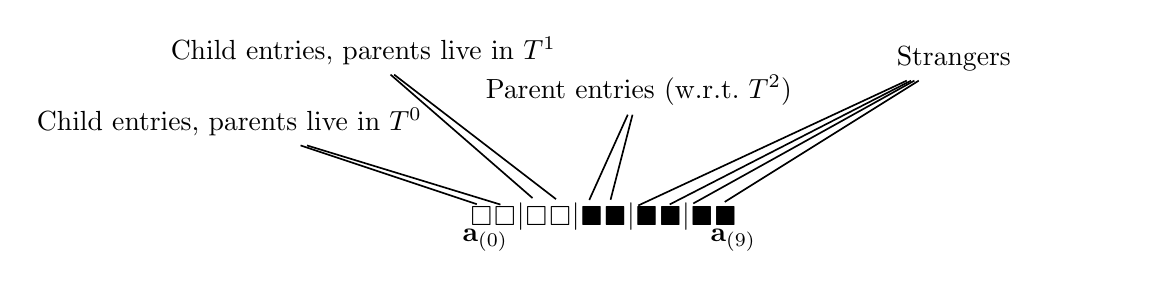
\begin{tikzpicture}[
  font=,
  to/.style={-,shorten >=1pt,semithick,font=\footnotesize}
	]


\node (box1) at (7, 0) {$\Box$};
\node (box2) at (7.3, 0) {$\Box$};
\node (line1) at (7.5, 0) {$\mid$};
\node (box3) at (7.7, 0) {$\Box$};
\node (box4) at (8.0, 0) {$\Box$};
\node (line2) at (8.2, 0) {$\mid$};
\node (box5) at (8.4, 0) {$\blacksquare$};
\node (box6) at (8.7, 0) {$\blacksquare$};
\node (line3) at (8.9, 0) {$\mid$};
\node (box7) at (9.1, 0) {$\blacksquare$};
\node (box8) at (9.4, 0) {$\blacksquare$};
\node (line4) at (9.6, 0) {$\mid$};
\node (box9) at (9.8, 0) {$\blacksquare$};
\node (box10) at (10.1, 0) {$\blacksquare$};

\node (rb1) at (7.1, 0.1) {};
\node (rb2) at (7.4, 0.1) {};

\node (rb3) at (7.8, 0.1) {};
\node (rb4) at (8.1, 0.1) {};

\node (rb5) at (8.3, 0.05) {};
\node (rb6) at (8.6, 0.05) {};

\node (ind1) at (7.05, -0.3) {$\vec{a}_{(0)}$};
\node (ind2) at (10.2, -0.3) {$\vec{a}_{(9)}$};

\node (label1) at (3.8, 1.2) {Child entries, parents live in $T^0$};
\node (label2) at (5.5, 2.1) {Child entries, parents live in $T^1$};
\node (label3) at (9, 1.6) {Parent entries (w.r.t.\ $T^2$)};
\node (label4) at (13, 2) {Strangers};

\draw[to] (label1) -- (rb1);
\draw[to] (label1) -- (rb2);

\draw[to] (label2) -- (rb3);
\draw[to] (label2) -- (rb4);

\draw[to] (label3) -- (rb5);
\draw[to] (label3) -- (rb6);

\draw[to] (label4) -- (box6);
\draw[to] (label4) -- (box7);
\draw[to] (label4) -- (box8);
\draw[to] (label4) -- (box9);

\node (dummy) at (15, 0) {};

\end{tikzpicture}
\hspace{\fill}
\caption{Children, parents and strangers.}
\label{fig:intuition}
\end{figure}}

\subsection{The Basic Idea}
For the general idea and intuition, assume $b=1$ and that $\shortvec{a}_{i}$ are outputs of $\Bdis{0}$ and we hence have $\Var(\shortvec{a}_{i,(0)}) = \sigma_r^2$. Now, some of these $\shortvec{a}_i$ will be stored in Table $T^1$ by $\Bdis{1}$ based on the value in the parent component $\shortvec{a}_{i,(1)}$. All future outputs of $\Bdis{1}$ which collide with $\shortvec{a}_{i}$ in the parent component at index 1 will have  $\shortvec{a}_i$ added/subtracted to it, we are hence adding a value with $\Var(\shortvec{a}_{i,(0)}) = \sigma_r^2$ in index 0.

Now, however, if the $\shortvec{a}_{i,(0)}$ happened to be unusually short, all $\Bdis{\ell}$ for $\ell > 0$ would output vectors with a shorter $\shortvec{a}_{i,(0)}$ added/subtracted in, i.e.\ would also have unusually small child components (although to a lesser degree). That is, improving the outputs of $\Bdis{1}$ -- i.e.\ decreasing the magnitude of the $\shortvec{a}_{i,(0)}$ stored in $T^1$ -- has a knock-on effect on all later outputs. More generally, improving the outputs of $\Bdis{\ell}$ will improve the outputs of $\Bdis{k}$ for $k>\ell$.

On the other hand, improving the outputs of $\Bdis{\ell}$ where $\ell$ is small, is easier than for larger values of $\ell$. In the algorithm as described so far, when we obtain a collision between a member of $T^\ell$ and an output $(\vec{a}_i, c_i)$ of $\Bdis{\ell-1}$, we reduce $(\vec{a}_i, c_i)$ using the colliding member of $T^\ell$, retaining this member in the table. Alternatively we can reduce $(\vec{a}_i, c_i)$ using the \emph{in-situ} table entry, replace the table entry with (the now reduced) $(\vec{a}_i, c_i)$ and return the former table entry as the output of $\Bdis{\ell}$. If we selectively employ this alternative strategy using the relative magnitudes of the child components of $(\vec{a}_i, c_i)$  and the table entry as a criterion, we can improve the `quality' of our tables as part of a pre-processing phase.

That is, in $\Bdis{\ell}$ for each collision in a parent component we may inspect the child components for their size and keep that in $T^\ell$ where the child components are smallest. Phrased in the language of `children' and `parents': we do not let `nature', i.e.\ randomness, run its course but intervene and select children based on their size. As the number of child components is $b \cdot \ell$ it becomes more difficult as $\ell$ increases to find vectors where all child components are short.

\subsection{Algorithms}
This leads to a modified algorithm $\Bdissm{\ell}$ given in Algorithm~\ref{alg:bdissmall}\submission{  which acts as a pre-processing phase.}{. Using Algorithms~\ref{alg:bdis} and \ref{alg:bdissmall} we may then present our revised version of the BKW algorithm in Algorithm~\ref{alg:bkw} where we first use Algorithm~\ref{alg:bdissmall} to produce `good' tables and then use Algorithm~\ref{alg:bdis} to sample $(\shortvec{a}_i,\tilde c_i)$ as before.}

\begin{algorithm}[H]
\label{alg:bdissmall}
\SetKw{KwAnd}{and}
\SetKw{KwOr}{or}
\SetKw{KwBreak}{break}
\submission{}{
\KwIn{$b$ -- an integer $0 < b \leq n$}
\KwIn{$\ell$ -- an integer $0 \leq \ell < a$}
\KwIn{$p$ -- an integer $0 < p \leq q$}
}
\Begin{
$T^{\ell} \gets$ table with $p^b$ rows maintained across all runs of ${\Bdissm{\ell}}$\;
Find $(\vec{a}',c') \gets T_{\vec{z}}^{\ell}$ that collides with a fresh sample $(\vec{a},c)$ from $\Bdis{\ell-1}$\submission{}{ as in Algorithm~\ref{alg:bdis}}\;

\If{$\sum_{i=0}^{b\cdot \ell -1} \abs{\vec{a}'_{(i)}} > \sum_{i=0}^{b\cdot \ell -1} \abs{\vec{a}_{(i)}}$}{
  $T^{\ell}_{\vec{z}} \gets (\vec{a},c)$\;
}
\Return $(\vec{a} - \vec{a}',c - c')$;
}
\caption{${\Bdissm{\ell}}$ for $0 \leq \ell < a$.}
\end{algorithm}

\submission{}{
\begin{algorithm}
\label{alg:bkw}
\SetKw{KwAnd}{and}
\SetKw{KwOr}{or}
\SetKw{KwBreak}{break}
 \KwIn{$b$ -- an integer $0 < b \leq n$}
 \KwIn{$a$ -- an integer such that $ab=n$}
 \KwIn{$p$ -- an integer $0 < p < q$}
 \KwIn{$o$ -- an integer $0 \leq o$}
\KwIn{$m$ -- an integer $0 \leq m$}
\
\Begin{
$o_t \gets o/(a+1)$\;
\tcp{populate elimination tables with random entries}
\For{$0 \leq i < o_t$} {
  $(\shortvec{a},c) \gets \Bdis{a-1}$; \tcp{$(\shortvec{a},c)$ is discarded}
}

\tcp{sample small entries}
\For{$0 \leq i < a$} {
  \For{$0 \leq j < o_t$} {
    $(\shortvec{a},c) \gets \Bdissm{i}$; \tcp{$(\shortvec{a},c)$ is discarded}
  }
}
\For{$0 \leq i < m$} {
  $(\shortvec{a}_i,c_i) \gets \Bdis{a-1}$\;
}
Run distinguisher on $c_i$ and return output\;
}
\caption{BKW with lazy modulus switching.}
\end{algorithm}}

\subsection{Picking $p$}
It remains to be established what the effect of such a strategy is, i.e.\ how fast children grow up or how fast rounding errors accumulate. 
In particular, given $n$ vectors $\vec{x}_i$ sampled from some distribution $\mathcal{D}$ where each component has standard deviation 
$\sigma$, i.e.\ $\Var(\vec{x}_{i,(j)}) = \sigma^2$ we are interested in the standard deviation $\sigma_{n}$ of each component for 
$\vec{x}^* = \min_{abs}\left(\vec{x}_0,\dots,\vec{x}_{n-1}\right)$ where $\min_{abs}$ picks that vector where 
$\sum_{j=0}^{b\cdot\ell-1} \abs{\vec{x}_{(j)}}$ is minimal. At this point we know no closed algebraic expression for $\sigma_n$. However, we found \submission{(as detailed in the full version of this work)}{ -- as detailed below -- }that $\sigma_n$ can be estimated as follows:
\begin{assumption}
\label{ass:minvar}
Let the vectors $\vec{x}_0,\ldots,\vec{x}_{n-1} \in \Z_q^{\tau}$ be sampled from some distribution $\mathcal{D}$ such that $\sigma^2 = \Var(\vec{x}_{i,(j)})$ where $\mathcal{D}$ is any distribution on (sub-)vectors observable in \submission{our algorithm}{Algorithm~\ref{alg:bkw}}. Let $\vec{x}^*=\min_{abs}\left(\vec{x}_0,\dots,\vec{x}_{n-1}\right)$ where $\min_{abs}$ picks that vector $\vec{x}^*$ with 
$\sum_{j=0}^{b\cdot\ell-1} \abs{\vec{x}^*_{(j)}}$ minimal. The stddev $\sigma_{n} = \sqrt{\Var(\vec{x}^*_{(0)})} =\cdots=\sqrt{\Var(\vec{x}^*_{(\tau-1)})}$ of components in $\vec{x}^*$ satisfies
$$\sigma/\sigma_n \geq c_\tau\, \sqrt[\tau]{n} + (1 - c_\tau)$$ with $c_\tau$ as in Table~\ref{tab:ctau} for $\tau \leq 10$ and 
$$c_\tau = 0.20151418166952917\,\sqrt{\tau}  + 0.32362108131969386\approx \frac{1}{5}\sqrt{\tau} + \frac{1}{3}$$
otherwise. 
\end{assumption}

\begin{table}
\centering\begin{footnotesize}
\begin{tabular}{|c|c|c|c|c|c|c|c|c|}
\hline
$\tau$    &         1  &         2  &         3  &         4  &         5\\
$c_\tau$  & 0.405799353869 & 0.692447899282 & 0.789885269135 & 0.844195936036 & 0.854967912468\\
\hline
$\tau$    &         6  &         7  &         8  &         9  &        10 \\
$c_\tau$  & 0.895446987232 & 0.91570933651 & 0.956763578012 & 0.943424544282 & 0.998715322134\\
\hline
\end{tabular}
\end{footnotesize}
\caption{$c_\tau$ for small values of $\tau$}
\label{tab:ctau}
\end{table}

\submission{}{We arrive at the approximation in Assumption~\ref{ass:minvar} as follows. We chose $\mathcal{D} = \U{\Z_{2^{32}}}$ and observed that $\sigma/\sigma_n$ behaves linearly when $\tau=1$ (cf.\ Figure~\ref{fig:sigman}). As we increase $\tau$ we expect the problem of finding short vectors to become exponentially harder. We also require $\sigma/\sigma_1 = 1$ for any $\tau$. The approximation $c_\tau \sqrt[\tau]{x} + (1 - c_\tau) = \sigma/\sigma_n$ satisfies all these conditions. Furthermore, experimental evidence suggests that there exist $c_\tau$ such that a function of this form approximates the observed data closely (cf.\ Figure~\ref{fig:sigman}). We then used curve fitting (as implemented in Sage~\cite{sagemath} via calls to SciPy \cite{scipy} which in turn calls MINPACK \cite{minpack}) on experimental data for $1 \leq n \leq 128$  to find $c_\tau$ for $1 \leq \tau \leq 512$; Table~\ref{tab:ctau} lists the first 10 such values. The expression $c_\tau \approx 1/5\sqrt{\tau} + 1/3$ was recovered by curve fitting the pairs $(1,c_1),\dots,(512,c_{512})$ recovered before (cf.\ Figure~\ref{fig:ctau} for a plot of this data and $1/5\sqrt{\tau}+1/3$). However, for small values of $\tau$ this expression diverges too much from the observed, which is why we are using explicit values instead. Finally, we assume that all distributions observed during the course of running our algorithm `shrink' at least as fast as the uniform distribution. An assumption we experimentally verified for the normal distribution and which seems to be confirmed by our experimental results in \submission{Appendix}{Section}~\ref{sec:implementation}.

\begin{figure}
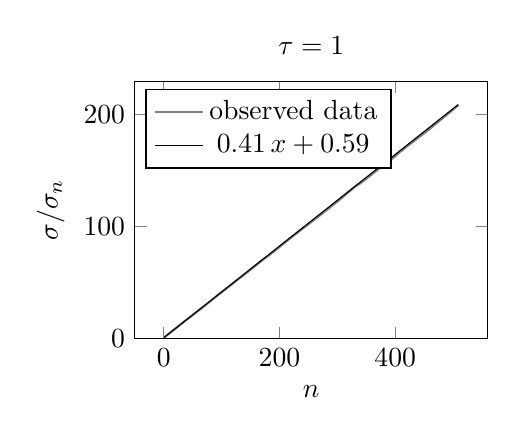
\begin{tikzpicture}
\pgfplotsset{width=.5\textwidth, height=0.4\textwidth}
\begin{axis}[xlabel={$n$},ylabel={$\sigma/\sigma_n$},ymin=0,legend pos=north west,title={$\tau=1$}]
\addplot[gray, thick] coordinates {
(  1, 1.00) (  5, 2.65) (  9, 4.28) ( 13, 5.92) ( 17, 7.54) ( 21, 9.19) ( 25, 10.83) ( 29, 12.47) ( 33, 14.12) ( 37, 15.74) ( 41, 17.29) ( 45, 18.85) ( 49, 20.47) ( 53, 22.09) ( 57, 23.66) ( 61, 25.26) ( 65, 26.90) ( 69, 28.51) ( 73, 30.15) ( 77, 31.68) ( 81, 33.40) ( 85, 35.10) ( 89, 36.76) ( 93, 38.42) ( 97, 40.08) (101, 41.65) (105, 43.30) (109, 44.88) (113, 46.45) (117, 48.11) (121, 49.75) (125, 51.44) (129, 52.95) (133, 54.59) (137, 56.11) (141, 57.80) (145, 59.43) (149, 61.10) (153, 62.87) (157, 64.42) (161, 65.98) (165, 67.66) (169, 69.38) (173, 70.93) (177, 72.38) (181, 73.84) (185, 75.44) (189, 77.15) (193, 78.82) (197, 80.39) (201, 82.06) (205, 83.86) (209, 85.52) (213, 87.10) (217, 88.90) (221, 90.51) (225, 92.10) (229, 93.56) (233, 95.28) (237, 96.95) (241, 98.50) (245, 99.97) (249, 101.53) (253, 103.17) (257, 104.83) (261, 106.45) (265, 107.99) (269, 109.59) (273, 111.15) (277, 112.88) (281, 114.50) (285, 116.00) (289, 117.74) (293, 119.46) (297, 121.11) (301, 122.61) (305, 124.36) (309, 126.10) (313, 127.76) (317, 129.59) (321, 131.37) (325, 133.03) (329, 134.78) (333, 136.20) (337, 137.62) (341, 138.94) (345, 140.53) (349, 142.17) (353, 143.88) (357, 145.41) (361, 147.05) (365, 148.81) (369, 150.39) (373, 151.86) (377, 153.50) (381, 155.20) (385, 156.69) (389, 158.30) (393, 159.90) (397, 161.37) (401, 163.14) (405, 165.11) (409, 166.87) (413, 168.28) (417, 170.09) (421, 171.64) (425, 173.41) (429, 174.83) (433, 176.39) (437, 178.15) (441, 179.67) (445, 181.29) (449, 182.80) (453, 184.30) (457, 185.98) (461, 187.66) (465, 189.26) (469, 191.24) (473, 192.74) (477, 194.53) (481, 196.21) (485, 197.99) (489, 199.71) (493, 201.31) (497, 203.03) (501, 204.80) (505, 206.53) (509, 208.03)

};
\addlegendentry{observed data}
\addplot[black] coordinates {
(  1, 1.00) (  5, 2.64) (  9, 4.27) ( 13, 5.91) ( 17, 7.55) ( 21, 9.18) ( 25, 10.82) ( 29, 12.45) ( 33, 14.09) ( 37, 15.73) ( 41, 17.36) ( 45, 19.00) ( 49, 20.64) ( 53, 22.27) ( 57, 23.91) ( 61, 25.54) ( 65, 27.18) ( 69, 28.82) ( 73, 30.45) ( 77, 32.09) ( 81, 33.73) ( 85, 35.36) ( 89, 37.00) ( 93, 38.63) ( 97, 40.27) (101, 41.91) (105, 43.54) (109, 45.18) (113, 46.82) (117, 48.45) (121, 50.09) (125, 51.73) (129, 53.36) (133, 55.00) (137, 56.63) (141, 58.27) (145, 59.91) (149, 61.54) (153, 63.18) (157, 64.82) (161, 66.45) (165, 68.09) (169, 69.72) (173, 71.36) (177, 73.00) (181, 74.63) (185, 76.27) (189, 77.91) (193, 79.54) (197, 81.18) (201, 82.82) (205, 84.45) (209, 86.09) (213, 87.72) (217, 89.36) (221, 91.00) (225, 92.63) (229, 94.27) (233, 95.91) (237, 97.54) (241, 99.18) (245, 100.81) (249, 102.45) (253, 104.09) (257, 105.72) (261, 107.36) (265, 109.00) (269, 110.63) (273, 112.27) (277, 113.90) (281, 115.54) (285, 117.18) (289, 118.81) (293, 120.45) (297, 122.09) (301, 123.72) (305, 125.36) (309, 127.00) (313, 128.63) (317, 130.27) (321, 131.90) (325, 133.54) (329, 135.18) (333, 136.81) (337, 138.45) (341, 140.09) (345, 141.72) (349, 143.36) (353, 144.99) (357, 146.63) (361, 148.27) (365, 149.90) (369, 151.54) (373, 153.18) (377, 154.81) (381, 156.45) (385, 158.09) (389, 159.72) (393, 161.36) (397, 162.99) (401, 164.63) (405, 166.27) (409, 167.90) (413, 169.54) (417, 171.18) (421, 172.81) (425, 174.45) (429, 176.08) (433, 177.72) (437, 179.36) (441, 180.99) (445, 182.63) (449, 184.27) (453, 185.90) (457, 187.54) (461, 189.17) (465, 190.81) (469, 192.45) (473, 194.08) (477, 195.72) (481, 197.36) (485, 198.99) (489, 200.63) (493, 202.27) (497, 203.90) (501, 205.54) (505, 207.17) (509, 208.81)
};
\addlegendentry{$0.41\, x + 0.59$}
\end{axis}
\end{tikzpicture}
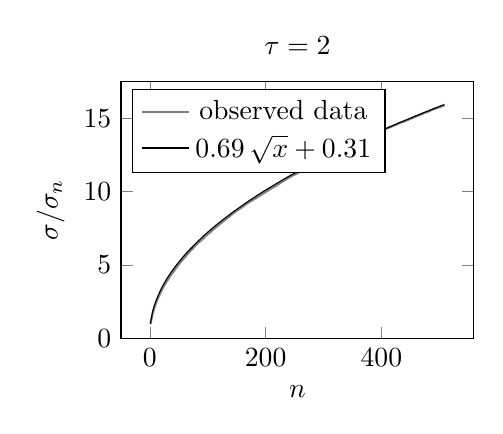
\begin{tikzpicture}
\pgfplotsset{width=.5\textwidth, height=0.4\textwidth}
\begin{axis}[xlabel={$n$},ylabel={$\sigma/\sigma_n$},ymin=0,legend pos=north west,title={$\tau=2$}]
\addplot[gray, thick] coordinates {
(  1, 1.00) (  5, 1.74) (  9, 2.23) ( 13, 2.65) ( 17, 3.01) ( 21, 3.34) ( 25, 3.63) ( 29, 3.88) ( 33, 4.12) ( 37, 4.36) ( 41, 4.57) ( 45, 4.78) ( 49, 5.00) ( 53, 5.20) ( 57, 5.38) ( 61, 5.56) ( 65, 5.74) ( 69, 5.92) ( 73, 6.08) ( 77, 6.25) ( 81, 6.41) ( 85, 6.56) ( 89, 6.70) ( 93, 6.84) ( 97, 7.00) (101, 7.13) (105, 7.26) (109, 7.41) (113, 7.54) (117, 7.66) (121, 7.80) (125, 7.92) (129, 8.04) (133, 8.17) (137, 8.29) (141, 8.43) (145, 8.55) (149, 8.67) (153, 8.77) (157, 8.88) (161, 8.99) (165, 9.12) (169, 9.22) (173, 9.32) (177, 9.41) (181, 9.51) (185, 9.60) (189, 9.70) (193, 9.80) (197, 9.90) (201, 10.00) (205, 10.10) (209, 10.20) (213, 10.29) (217, 10.37) (221, 10.48) (225, 10.58) (229, 10.68) (233, 10.78) (237, 10.88) (241, 10.97) (245, 11.06) (249, 11.14) (253, 11.22) (257, 11.31) (261, 11.39) (265, 11.47) (269, 11.55) (273, 11.63) (277, 11.72) (281, 11.81) (285, 11.89) (289, 11.99) (293, 12.08) (297, 12.16) (301, 12.25) (305, 12.33) (309, 12.42) (313, 12.50) (317, 12.58) (321, 12.65) (325, 12.73) (329, 12.80) (333, 12.88) (337, 12.96) (341, 13.04) (345, 13.12) (349, 13.19) (353, 13.27) (357, 13.34) (361, 13.42) (365, 13.50) (369, 13.57) (373, 13.65) (377, 13.72) (381, 13.79) (385, 13.86) (389, 13.94) (393, 14.00) (397, 14.08) (401, 14.14) (405, 14.22) (409, 14.30) (413, 14.36) (417, 14.42) (421, 14.49) (425, 14.56) (429, 14.64) (433, 14.69) (437, 14.75) (441, 14.80) (445, 14.87) (449, 14.94) (453, 15.00) (457, 15.07) (461, 15.14) (465, 15.20) (469, 15.27) (473, 15.34) (477, 15.40) (481, 15.45) (485, 15.53) (489, 15.60) (493, 15.66) (497, 15.71) (501, 15.76) (505, 15.81) (509, 15.88)
};
\addlegendentry{observed data}
\addplot[black,smooth] coordinates {
(  1, 1.00) (  5, 1.86) (  9, 2.38) ( 13, 2.80) ( 17, 3.16) ( 21, 3.48) ( 25, 3.77) ( 29, 4.04) ( 33, 4.29) ( 37, 4.52) ( 41, 4.74) ( 45, 4.95) ( 49, 5.15) ( 53, 5.35) ( 57, 5.54) ( 61, 5.72) ( 65, 5.89) ( 69, 6.06) ( 73, 6.22) ( 77, 6.38) ( 81, 6.54) ( 85, 6.69) ( 89, 6.84) ( 93, 6.99) ( 97, 7.13) (101, 7.27) (105, 7.40) (109, 7.54) (113, 7.67) (117, 7.80) (121, 7.92) (125, 8.05) (129, 8.17) (133, 8.29) (137, 8.41) (141, 8.53) (145, 8.65) (149, 8.76) (153, 8.87) (157, 8.98) (161, 9.09) (165, 9.20) (169, 9.31) (173, 9.42) (177, 9.52) (181, 9.62) (185, 9.73) (189, 9.83) (193, 9.93) (197, 10.03) (201, 10.12) (205, 10.22) (209, 10.32) (213, 10.41) (217, 10.51) (221, 10.60) (225, 10.69) (229, 10.79) (233, 10.88) (237, 10.97) (241, 11.06) (245, 11.15) (249, 11.23) (253, 11.32) (257, 11.41) (261, 11.49) (265, 11.58) (269, 11.66) (273, 11.75) (277, 11.83) (281, 11.92) (285, 12.00) (289, 12.08) (293, 12.16) (297, 12.24) (301, 12.32) (305, 12.40) (309, 12.48) (313, 12.56) (317, 12.64) (321, 12.71) (325, 12.79) (329, 12.87) (333, 12.94) (337, 13.02) (341, 13.09) (345, 13.17) (349, 13.24) (353, 13.32) (357, 13.39) (361, 13.46) (365, 13.54) (369, 13.61) (373, 13.68) (377, 13.75) (381, 13.82) (385, 13.89) (389, 13.96) (393, 14.03) (397, 14.10) (401, 14.17) (405, 14.24) (409, 14.31) (413, 14.38) (417, 14.45) (421, 14.52) (425, 14.58) (429, 14.65) (433, 14.72) (437, 14.78) (441, 14.85) (445, 14.91) (449, 14.98) (453, 15.05) (457, 15.11) (461, 15.18) (465, 15.24) (469, 15.30) (473, 15.37) (477, 15.43) (481, 15.49) (485, 15.56) (489, 15.62) (493, 15.68) (497, 15.74) (501, 15.81) (505, 15.87) (509, 15.93)
};
\addlegendentry{$0.69\, \sqrt{x} + 0.31$}
\end{axis}
\end{tikzpicture}\\

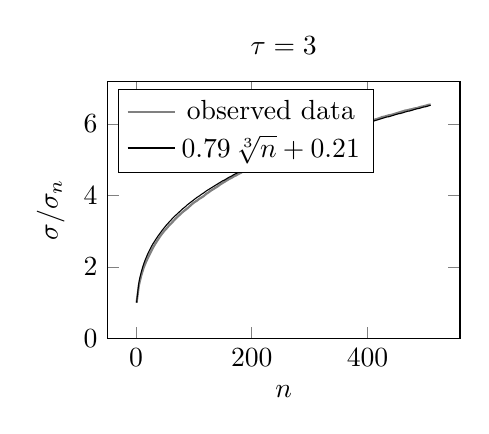
\begin{tikzpicture}
\pgfplotsset{width=.5\textwidth, height=0.4\textwidth}
\begin{axis}[xlabel={$n$},ylabel={$\sigma/\sigma_n$},ymin=0,legend pos=north west,title={$\tau=3$}]
\addplot[gray, thick] coordinates {
(  1, 1.00) (  5, 1.49) (  9, 1.76) ( 13, 1.97) ( 17, 2.13) ( 21, 2.27) ( 25, 2.40) ( 29, 2.53) ( 33, 2.64) ( 37, 2.74) ( 41, 2.84) ( 45, 2.93) ( 49, 3.01) ( 53, 3.08) ( 57, 3.16) ( 61, 3.22) ( 65, 3.29) ( 69, 3.36) ( 73, 3.42) ( 77, 3.48) ( 81, 3.54) ( 85, 3.59) ( 89, 3.64) ( 93, 3.70) ( 97, 3.76) (101, 3.81) (105, 3.85) (109, 3.90) (113, 3.94) (117, 3.98) (121, 4.04) (125, 4.08) (129, 4.13) (133, 4.17) (137, 4.21) (141, 4.25) (145, 4.30) (149, 4.34) (153, 4.38) (157, 4.42) (161, 4.46) (165, 4.49) (169, 4.53) (173, 4.56) (177, 4.60) (181, 4.63) (185, 4.67) (189, 4.71) (193, 4.74) (197, 4.77) (201, 4.80) (205, 4.84) (209, 4.87) (213, 4.90) (217, 4.93) (221, 4.96) (225, 4.99) (229, 5.03) (233, 5.05) (237, 5.08) (241, 5.11) (245, 5.14) (249, 5.17) (253, 5.20) (257, 5.23) (261, 5.26) (265, 5.29) (269, 5.31) (273, 5.35) (277, 5.37) (281, 5.40) (285, 5.42) (289, 5.45) (293, 5.47) (297, 5.49) (301, 5.52) (305, 5.54) (309, 5.56) (313, 5.58) (317, 5.61) (321, 5.63) (325, 5.65) (329, 5.69) (333, 5.71) (337, 5.73) (341, 5.76) (345, 5.78) (349, 5.80) (353, 5.82) (357, 5.84) (361, 5.86) (365, 5.88) (369, 5.90) (373, 5.93) (377, 5.95) (381, 5.96) (385, 5.98) (389, 6.00) (393, 6.02) (397, 6.04) (401, 6.06) (405, 6.08) (409, 6.10) (413, 6.12) (417, 6.14) (421, 6.16) (425, 6.19) (429, 6.20) (433, 6.22) (437, 6.24) (441, 6.25) (445, 6.27) (449, 6.29) (453, 6.31) (457, 6.33) (461, 6.35) (465, 6.37) (469, 6.38) (473, 6.40) (477, 6.41) (481, 6.43) (485, 6.44) (489, 6.46) (493, 6.48) (497, 6.49) (501, 6.51) (505, 6.53) (509, 6.54)
};
\addlegendentry{observed data}
\addplot[black,smooth] coordinates {
(  1, 1.00) (  5, 1.56) (  9, 1.85) ( 13, 2.07) ( 17, 2.24) ( 21, 2.39) ( 25, 2.52) ( 29, 2.64) ( 33, 2.74) ( 37, 2.84) ( 41, 2.93) ( 45, 3.02) ( 49, 3.10) ( 53, 3.18) ( 57, 3.25) ( 61, 3.32) ( 65, 3.39) ( 69, 3.45) ( 73, 3.51) ( 77, 3.57) ( 81, 3.63) ( 85, 3.68) ( 89, 3.74) ( 93, 3.79) ( 97, 3.84) (101, 3.89) (105, 3.94) (109, 3.98) (113, 4.03) (117, 4.07) (121, 4.12) (125, 4.16) (129, 4.20) (133, 4.24) (137, 4.28) (141, 4.32) (145, 4.36) (149, 4.40) (153, 4.43) (157, 4.47) (161, 4.51) (165, 4.54) (169, 4.58) (173, 4.61) (177, 4.65) (181, 4.68) (185, 4.71) (189, 4.74) (193, 4.77) (197, 4.81) (201, 4.84) (205, 4.87) (209, 4.90) (213, 4.93) (217, 4.96) (221, 4.99) (225, 5.01) (229, 5.04) (233, 5.07) (237, 5.10) (241, 5.13) (245, 5.15) (249, 5.18) (253, 5.21) (257, 5.23) (261, 5.26) (265, 5.28) (269, 5.31) (273, 5.33) (277, 5.36) (281, 5.38) (285, 5.41) (289, 5.43) (293, 5.46) (297, 5.48) (301, 5.50) (305, 5.53) (309, 5.55) (313, 5.57) (317, 5.60) (321, 5.62) (325, 5.64) (329, 5.66) (333, 5.69) (337, 5.71) (341, 5.73) (345, 5.75) (349, 5.77) (353, 5.79) (357, 5.81) (361, 5.83) (365, 5.86) (369, 5.88) (373, 5.90) (377, 5.92) (381, 5.94) (385, 5.96) (389, 5.98) (393, 6.00) (397, 6.02) (401, 6.03) (405, 6.05) (409, 6.07) (413, 6.09) (417, 6.11) (421, 6.13) (425, 6.15) (429, 6.17) (433, 6.19) (437, 6.20) (441, 6.22) (445, 6.24) (449, 6.26) (453, 6.28) (457, 6.29) (461, 6.31) (465, 6.33) (469, 6.35) (473, 6.36) (477, 6.38) (481, 6.40) (485, 6.42) (489, 6.43) (493, 6.45) (497, 6.47) (501, 6.48) (505, 6.50) (509, 6.52)
};
\addlegendentry{$0.79\, \sqrt[3]{n} +  0.21$}
\end{axis}
\end{tikzpicture}
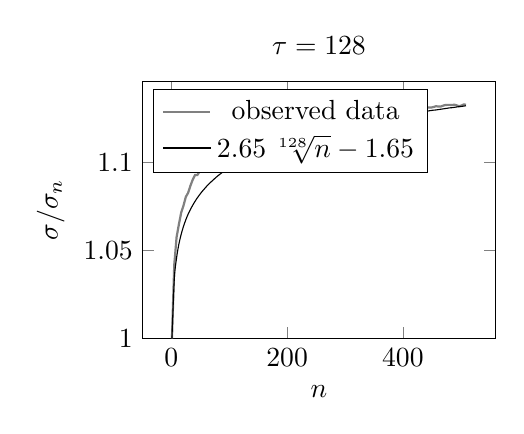
\begin{tikzpicture}
\pgfplotsset{width=.5\textwidth, height=0.4\textwidth}
\begin{axis}[xlabel={$n$},ylabel={$\sigma/\sigma_n$},ymin=1,legend pos=north west,title={$\tau=128$}]
\addplot[gray, thick] coordinates {
(  1, 1.0000) (  5, 1.0418) (  9, 1.0575) ( 13, 1.0648) ( 17, 1.0715) ( 21, 1.0755) ( 25, 1.0804) ( 29, 1.0827) ( 33, 1.0868) ( 37, 1.0902) ( 41, 1.0928) ( 45, 1.0928) ( 49, 1.0949) ( 53, 1.0968) ( 57, 1.0983) ( 61, 1.0992) ( 65, 1.1007) ( 69, 1.1013) ( 73, 1.1024) ( 77, 1.1033) ( 81, 1.1043) ( 85, 1.1057) ( 89, 1.1049) ( 93, 1.1054) ( 97, 1.1057) (101, 1.1066) (105, 1.1074) (109, 1.1080) (113, 1.1094) (117, 1.1102) (121, 1.1100) (125, 1.1109) (129, 1.1101) (133, 1.1113) (137, 1.1120) (141, 1.1128) (145, 1.1132) (149, 1.1138) (153, 1.1142) (157, 1.1140) (161, 1.1137) (165, 1.1136) (169, 1.1151) (173, 1.1150) (177, 1.1149) (181, 1.1155) (185, 1.1158) (189, 1.1162) (193, 1.1166) (197, 1.1169) (201, 1.1176) (205, 1.1172) (209, 1.1173) (213, 1.1172) (217, 1.1179) (221, 1.1189) (225, 1.1195) (229, 1.1193) (233, 1.1198) (237, 1.1210) (241, 1.1216) (245, 1.1220) (249, 1.1220) (253, 1.1215) (257, 1.1219) (261, 1.1222) (265, 1.1226) (269, 1.1230) (273, 1.1238) (277, 1.1246) (281, 1.1248) (285, 1.1255) (289, 1.1258) (293, 1.1252) (297, 1.1253) (301, 1.1251) (305, 1.1253) (309, 1.1259) (313, 1.1262) (317, 1.1265) (321, 1.1267) (325, 1.1268) (329, 1.1268) (333, 1.1264) (337, 1.1272) (341, 1.1272) (345, 1.1267) (349, 1.1269) (353, 1.1270) (357, 1.1273) (361, 1.1277) (365, 1.1275) (369, 1.1272) (373, 1.1275) (377, 1.1273) (381, 1.1272) (385, 1.1273) (389, 1.1270) (393, 1.1274) (397, 1.1280) (401, 1.1286) (405, 1.1291) (409, 1.1295) (413, 1.1296) (417, 1.1299) (421, 1.1300) (425, 1.1303) (429, 1.1306) (433, 1.1309) (437, 1.1312) (441, 1.1311) (445, 1.1311) (449, 1.1311) (453, 1.1314) (457, 1.1318) (461, 1.1317) (465, 1.1316) (469, 1.1321) (473, 1.1325) (477, 1.1326) (481, 1.1326) (485, 1.1325) (489, 1.1327) (493, 1.1323) (497, 1.1318) (501, 1.1322) (505, 1.1328) (509, 1.1327)
};
\addlegendentry{observed data}
\addplot[black,smooth] coordinates {
(  1, 1.0000) (  5, 1.0335) (  9, 1.0458) ( 13, 1.0536) ( 17, 1.0592) ( 21, 1.0637) ( 25, 1.0674) ( 29, 1.0706) ( 33, 1.0733) ( 37, 1.0757) ( 41, 1.0779) ( 45, 1.0799) ( 49, 1.0817) ( 53, 1.0834) ( 57, 1.0849) ( 61, 1.0864) ( 65, 1.0878) ( 69, 1.0890) ( 73, 1.0902) ( 77, 1.0914) ( 81, 1.0925) ( 85, 1.0935) ( 89, 1.0945) ( 93, 1.0954) ( 97, 1.0963) (101, 1.0972) (105, 1.0980) (109, 1.0988) (113, 1.0996) (117, 1.1003) (121, 1.1011) (125, 1.1018) (129, 1.1024) (133, 1.1031) (137, 1.1037) (141, 1.1043) (145, 1.1050) (149, 1.1055) (153, 1.1061) (157, 1.1067) (161, 1.1072) (165, 1.1077) (169, 1.1082) (173, 1.1087) (177, 1.1092) (181, 1.1097) (185, 1.1102) (189, 1.1107) (193, 1.1111) (197, 1.1115) (201, 1.1120) (205, 1.1124) (209, 1.1128) (213, 1.1132) (217, 1.1136) (221, 1.1140) (225, 1.1144) (229, 1.1148) (233, 1.1152) (237, 1.1155) (241, 1.1159) (245, 1.1163) (249, 1.1166) (253, 1.1169) (257, 1.1173) (261, 1.1176) (265, 1.1179) (269, 1.1183) (273, 1.1186) (277, 1.1189) (281, 1.1192) (285, 1.1195) (289, 1.1198) (293, 1.1201) (297, 1.1204) (301, 1.1207) (305, 1.1210) (309, 1.1213) (313, 1.1215) (317, 1.1218) (321, 1.1221) (325, 1.1224) (329, 1.1226) (333, 1.1229) (337, 1.1231) (341, 1.1234) (345, 1.1237) (349, 1.1239) (353, 1.1241) (357, 1.1244) (361, 1.1246) (365, 1.1249) (369, 1.1251) (373, 1.1253) (377, 1.1256) (381, 1.1258) (385, 1.1260) (389, 1.1262) (393, 1.1265) (397, 1.1267) (401, 1.1269) (405, 1.1271) (409, 1.1273) (413, 1.1275) (417, 1.1278) (421, 1.1280) (425, 1.1282) (429, 1.1284) (433, 1.1286) (437, 1.1288) (441, 1.1290) (445, 1.1292) (449, 1.1294) (453, 1.1296) (457, 1.1297) (461, 1.1299) (465, 1.1301) (469, 1.1303) (473, 1.1305) (477, 1.1307) (481, 1.1309) (485, 1.1310) (489, 1.1312) (493, 1.1314) (497, 1.1316) (501, 1.1317) (505, 1.1319) (509, 1.1321)
};
\addlegendentry{$2.65\,\sqrt[128]{n} -1.65$}
\end{axis}
\end{tikzpicture}
\caption{$\sigma/\sigma_n$ for $1 \leq \tau \leq 3$ and $\tau = 128$.}
\label{fig:sigman}
\end{figure}

\begin{figure}
\centering
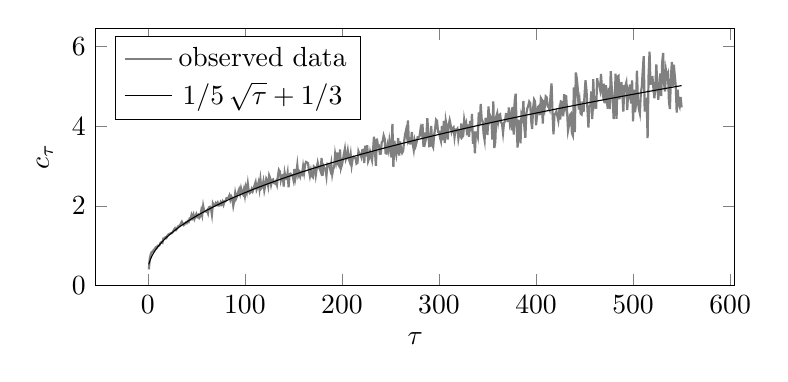
\begin{tikzpicture}
\pgfplotsset{width=.8\textwidth, height=0.4\textwidth}
\begin{axis}[xlabel={$\tau$},ylabel={$c_\tau$},ymin=0,legend pos=north west]
\addplot[gray, thick] coordinates {
(  1,0.4058) (  2,0.6924) (  3,0.7899) (  4,0.8442) (  5,0.8550) (  6,0.8954) (  7,0.9157) (  8,0.9568) (  9,0.9434) ( 10,0.9987) ( 11,0.9938) ( 12,1.0161) ( 13,1.0731) ( 14,1.0919) ( 15,1.0759) ( 16,1.1823) ( 17,1.1774) ( 18,1.2120) ( 19,1.1974) ( 20,1.2487) ( 21,1.2782) ( 22,1.2985) ( 23,1.3073) ( 24,1.3130) ( 25,1.3209) ( 26,1.3607) ( 27,1.4055) ( 28,1.4394) ( 29,1.3987) ( 30,1.4313) ( 31,1.4850) ( 32,1.4991) ( 33,1.5145) ( 34,1.5562) ( 35,1.6032) ( 36,1.5585) ( 37,1.5213) ( 38,1.5481) ( 39,1.5811) ( 40,1.5668) ( 41,1.6162) ( 42,1.5995) ( 43,1.6806) ( 44,1.6655) ( 45,1.7726) ( 46,1.7071) ( 47,1.7799) ( 48,1.6747) ( 49,1.7351) ( 50,1.7976) ( 51,1.7312) ( 52,1.7667) ( 53,1.7028) ( 54,1.7445) ( 55,1.8793) ( 56,1.7712) ( 57,1.9964) ( 58,1.8654) ( 59,1.8702) ( 60,1.8592) ( 61,1.8924) ( 62,1.8184) ( 63,1.9655) ( 64,1.9782) ( 65,1.9418) ( 66,1.7854) ( 67,2.0597) ( 68,2.0057) ( 69,2.0127) ( 70,2.0715) ( 71,2.0337) ( 72,2.0822) ( 73,2.0125) ( 74,2.0165) ( 75,2.0925) ( 76,2.0462) ( 77,2.1064) ( 78,2.0311) ( 79,2.1135) ( 80,2.1172) ( 81,2.1969) ( 82,2.1995) ( 83,2.1995) ( 84,2.2615) ( 85,2.1548) ( 86,2.2348) ( 87,2.1860) ( 88,2.0046) ( 89,2.1310) ( 90,2.3220) ( 91,2.1925) ( 92,2.2525) ( 93,2.3475) ( 94,2.4155) ( 95,2.3092) ( 96,2.4449) ( 97,2.3501) ( 98,2.2988) ( 99,2.4143) (100,2.2617) (101,2.4649) (102,2.3594) (103,2.5571) (104,2.3710) (105,2.3250) (106,2.3475) (107,2.4261) (108,2.3702) (109,2.4468) (110,2.5229) (111,2.5984) (112,2.4161) (113,2.4865) (114,2.5863) (115,2.4243) (116,2.6603) (117,2.4491) (118,2.4805) (119,2.6085) (120,2.3955) (121,2.5182) (122,2.6857) (123,2.6341) (124,2.5049) (125,2.7653) (126,2.6996) (127,2.5355) (128,2.6471) (129,2.6648) (130,2.5792) (131,2.5628) (132,2.6139) (133,2.5319) (134,2.7467) (135,2.9048) (136,2.8649) (137,2.6512) (138,2.7611) (139,2.7748) (140,2.4852) (141,2.8236) (142,2.6930) (143,2.6825) (144,2.8289) (145,2.4715) (146,2.7951) (147,2.8104) (148,2.7720) (149,2.7693) (150,2.6601) (151,2.9308) (152,2.6932) (153,2.8181) (154,3.0256) (155,2.7691) (156,2.8357) (157,2.7425) (158,2.8379) (159,2.8025) (160,2.9963) (161,2.8434) (162,3.0370) (163,3.1057) (164,3.0928) (165,3.0772) (166,2.8924) (167,2.7545) (168,2.8885) (169,2.7534) (170,2.7250) (171,2.9911) (172,2.9668) (173,2.7708) (174,2.9412) (175,3.0837) (176,2.9726) (177,2.9411) (178,2.8720) (179,3.2077) (180,2.7599) (181,3.0064) (182,2.9511) (183,2.9271) (184,2.7552) (185,3.0595) (186,3.0542) (187,3.0022) (188,2.9071) (189,3.0659) (190,2.7977) (191,2.9342) (192,2.9744) (193,3.2930) (194,3.1383) (195,3.3462) (196,3.0510) (197,3.0103) (198,3.4188) (199,2.9526) (200,3.0363) (201,3.1650) (202,3.3040) (203,3.4317) (204,3.1735) (205,3.2419) (206,3.3863) (207,3.1916) (208,3.1180) (209,3.2886) (210,3.0246) (211,3.1816) (212,3.2318) (213,3.2093) (214,3.2081) (215,3.0641) (216,3.0826) (217,3.3742) (218,3.3111) (219,3.3047) (220,3.2311) (221,3.4045) (222,3.4104) (223,3.0798) (224,3.5115) (225,3.2421) (226,3.5253) (227,3.1273) (228,3.1978) (229,3.3573) (230,3.2542) (231,3.1501) (232,3.3897) (233,3.7380) (234,3.3810) (235,3.0094) (236,3.6927) (237,3.5303) (238,3.5248) (239,3.3114) (240,3.3164) (241,3.6042) (242,3.6269) (243,3.7673) (244,3.6863) (245,3.3243) (246,3.3171) (247,3.5231) (248,3.4024) (249,3.6509) (250,3.5084) (251,3.2150) (252,4.0597) (253,2.9809) (254,3.6406) (255,3.4320) (256,3.2856) (257,3.4825) (258,3.7053) (259,3.2690) (260,3.6193) (261,3.4070) (262,3.3311) (263,3.3781) (264,3.6063) (265,3.7880) (266,3.8970) (267,3.7489) (268,4.1503) (269,3.5818) (270,3.5700) (271,3.5723) (272,3.8611) (273,3.5485) (274,3.4078) (275,3.6321) (276,3.5150) (277,3.6080) (278,3.7252) (279,3.7233) (280,3.7535) (281,3.9294) (282,3.8313) (283,4.0628) (284,3.4847) (285,3.8481) (286,3.6244) (287,3.7337) (288,4.2035) (289,3.8063) (290,3.5031) (291,3.5120) (292,4.0115) (293,3.5387) (294,3.4775) (295,3.7822) (296,3.9315) (297,4.1665) (298,4.1399) (299,3.8672) (300,3.8672) (301,3.7306) (302,3.6350) (303,4.0078) (304,3.6467) (305,4.1349) (306,3.5797) (307,4.1308) (308,3.9833) (309,3.6674) (310,4.0381) (311,4.1560) (312,4.0384) (313,3.8639) (314,3.9418) (315,3.9728) (316,3.7298) (317,3.9182) (318,3.9104) (319,3.9420) (320,3.6933) (321,3.8387) (322,3.7795) (323,4.0712) (324,3.7330) (325,3.7661) (326,4.1626) (327,4.0156) (328,4.0843) (329,3.7733) (330,4.0472) (331,3.7384) (332,4.1354) (333,3.8730) (334,4.3096) (335,3.5634) (336,3.8694) (337,3.3225) (338,3.8471) (339,3.8450) (340,3.7432) (341,4.3481) (342,4.0332) (343,4.5624) (344,4.1792) (345,4.1220) (346,3.8054) (347,3.6587) (348,4.2143) (349,4.0000) (350,3.7824) (351,4.4978) (352,4.1524) (353,4.2483) (354,4.1832) (355,3.6698) (356,4.6249) (357,3.4559) (358,3.5974) (359,4.2480) (360,4.3294) (361,4.1170) (362,4.2840) (363,4.3022) (364,4.0992) (365,4.0547) (366,3.8371) (367,4.0896) (368,4.1209) (369,4.3082) (370,4.3021) (371,4.1068) (372,4.4740) (373,4.1115) (374,4.2475) (375,3.9018) (376,4.4886) (377,3.7951) (378,4.6358) (379,4.8218) (380,3.9993) (381,3.4680) (382,4.1694) (383,3.9079) (384,3.5750) (385,4.2867) (386,4.2083) (387,4.6371) (388,3.9796) (389,3.7109) (390,4.3172) (391,4.4475) (392,4.5146) (393,4.6199) (394,4.5796) (395,4.1412) (396,3.9349) (397,4.4529) (398,4.6733) (399,4.6252) (400,4.0269) (401,4.2651) (402,4.4856) (403,4.5120) (404,4.2815) (405,4.7098) (406,4.6674) (407,4.0705) (408,4.6623) (409,4.4974) (410,4.7534) (411,4.7294) (412,4.5015) (413,4.4831) (414,4.4196) (415,4.7875) (416,5.0807) (417,4.3471) (418,3.8005) (419,4.2955) (420,4.3206) (421,4.3761) (422,4.2592) (423,4.1436) (424,4.3861) (425,4.1702) (426,4.6201) (427,4.6056) (428,4.2540) (429,4.8066) (430,4.5605) (431,4.7794) (432,4.3919) (433,3.9010) (434,4.0365) (435,4.2852) (436,4.3166) (437,3.8298) (438,3.7692) (439,4.9795) (440,3.8529) (441,5.3523) (442,5.2106) (443,4.9521) (444,4.4222) (445,4.6123) (446,4.3176) (447,4.2975) (448,4.6281) (449,4.3599) (450,4.7855) (451,5.1565) (452,4.9128) (453,4.4298) (454,3.9686) (455,4.4866) (456,4.5406) (457,4.8752) (458,4.1834) (459,5.1880) (460,4.5173) (461,4.5960) (462,4.4445) (463,5.2100) (464,5.0413) (465,5.0396) (466,4.9248) (467,5.3160) (468,4.8926) (469,4.7740) (470,5.0689) (471,4.5787) (472,5.0332) (473,4.6134) (474,4.4451) (475,4.9686) (476,4.4332) (477,5.3870) (478,4.9918) (479,4.6935) (480,4.1822) (481,4.5083) (482,5.3241) (483,4.1917) (484,5.2480) (485,5.2678) (486,4.6813) (487,4.8442) (488,5.1125) (489,4.7816) (490,4.3691) (491,5.0093) (492,5.0051) (493,5.0952) (494,4.4074) (495,4.8943) (496,4.8039) (497,5.0544) (498,4.5712) (499,5.1556) (500,4.1257) (501,4.9230) (502,4.3524) (503,4.5519) (504,5.4003) (505,4.6430) (506,4.4364) (507,4.3248) (508,4.8291) (509,4.9893) (510,5.4051) (511,5.7646) (512,4.3736) (513,4.6343) (514,4.6742) (515,3.7062) (516,5.2851) (517,5.8774) (518,5.0435) (519,5.2224) (520,5.2345) (521,4.9534) (522,4.7044) (523,5.0074) (524,5.5556) (525,5.0152) (526,4.6688) (527,4.9707) (528,5.3267) (529,4.7606) (530,5.6030) (531,5.8456) (532,5.0616) (533,4.8779) (534,5.3991) (535,5.2488) (536,5.3211) (537,4.6155) (538,4.4361) (539,5.2254) (540,5.6167) (541,5.0042) (542,5.5512) (543,5.2675) (544,5.0142) (545,4.3433) (546,4.9208) (547,4.5879) (548,4.5061) (549,4.7379) (550,4.4772)
};
\addlegendentry{observed data}
\addplot[black,smooth] coordinates {(  1,0.5333) (  2,0.6162) (  3,0.6797) (  4,0.7333) (  5,0.7805) (  6,0.8232) (  7,0.8625) (  8,0.8990) (  9,0.9333) ( 10,0.9658) ( 11,0.9967) ( 12,1.0262) ( 13,1.0544) ( 14,1.0817) ( 15,1.1079) ( 16,1.1333) ( 17,1.1580) ( 18,1.1819) ( 19,1.2051) ( 20,1.2278) ( 21,1.2498) ( 22,1.2714) ( 23,1.2925) ( 24,1.3131) ( 25,1.3333) ( 26,1.3531) ( 27,1.3726) ( 28,1.3916) ( 29,1.4104) ( 30,1.4288) ( 31,1.4469) ( 32,1.4647) ( 33,1.4822) ( 34,1.4995) ( 35,1.5165) ( 36,1.5333) ( 37,1.5499) ( 38,1.5662) ( 39,1.5823) ( 40,1.5982) ( 41,1.6140) ( 42,1.6295) ( 43,1.6448) ( 44,1.6600) ( 45,1.6750) ( 46,1.6898) ( 47,1.7045) ( 48,1.7190) ( 49,1.7333) ( 50,1.7475) ( 51,1.7616) ( 52,1.7756) ( 53,1.7894) ( 54,1.8030) ( 55,1.8166) ( 56,1.8300) ( 57,1.8433) ( 58,1.8565) ( 59,1.8696) ( 60,1.8825) ( 61,1.8954) ( 62,1.9081) ( 63,1.9208) ( 64,1.9333) ( 65,1.9458) ( 66,1.9581) ( 67,1.9704) ( 68,1.9826) ( 69,1.9947) ( 70,2.0067) ( 71,2.0186) ( 72,2.0304) ( 73,2.0421) ( 74,2.0538) ( 75,2.0654) ( 76,2.0769) ( 77,2.0883) ( 78,2.0997) ( 79,2.1110) ( 80,2.1222) ( 81,2.1333) ( 82,2.1444) ( 83,2.1554) ( 84,2.1664) ( 85,2.1772) ( 86,2.1881) ( 87,2.1988) ( 88,2.2095) ( 89,2.2201) ( 90,2.2307) ( 91,2.2412) ( 92,2.2517) ( 93,2.2621) ( 94,2.2724) ( 95,2.2827) ( 96,2.2929) ( 97,2.3031) ( 98,2.3132) ( 99,2.3233) (100,2.3333) (101,2.3433) (102,2.3532) (103,2.3631) (104,2.3729) (105,2.3827) (106,2.3925) (107,2.4021) (108,2.4118) (109,2.4214) (110,2.4310) (111,2.4405) (112,2.4499) (113,2.4594) (114,2.4687) (115,2.4781) (116,2.4874) (117,2.4967) (118,2.5059) (119,2.5151) (120,2.5242) (121,2.5333) (122,2.5424) (123,2.5514) (124,2.5604) (125,2.5694) (126,2.5783) (127,2.5872) (128,2.5961) (129,2.6049) (130,2.6137) (131,2.6224) (132,2.6312) (133,2.6398) (134,2.6485) (135,2.6571) (136,2.6657) (137,2.6743) (138,2.6828) (139,2.6913) (140,2.6998) (141,2.7082) (142,2.7166) (143,2.7250) (144,2.7333) (145,2.7417) (146,2.7499) (147,2.7582) (148,2.7664) (149,2.7746) (150,2.7828) (151,2.7910) (152,2.7991) (153,2.8072) (154,2.8153) (155,2.8233) (156,2.8313) (157,2.8393) (158,2.8473) (159,2.8552) (160,2.8632) (161,2.8710) (162,2.8789) (163,2.8868) (164,2.8946) (165,2.9024) (166,2.9102) (167,2.9179) (168,2.9256) (169,2.9333) (170,2.9410) (171,2.9487) (172,2.9563) (173,2.9639) (174,2.9715) (175,2.9791) (176,2.9866) (177,2.9942) (178,3.0017) (179,3.0092) (180,3.0166) (181,3.0241) (182,3.0315) (183,3.0389) (184,3.0463) (185,3.0536) (186,3.0610) (187,3.0683) (188,3.0756) (189,3.0829) (190,3.0901) (191,3.0974) (192,3.1046) (193,3.1118) (194,3.1190) (195,3.1262) (196,3.1333) (197,3.1405) (198,3.1476) (199,3.1547) (200,3.1618) (201,3.1688) (202,3.1759) (203,3.1829) (204,3.1899) (205,3.1969) (206,3.2039) (207,3.2108) (208,3.2178) (209,3.2247) (210,3.2316) (211,3.2385) (212,3.2454) (213,3.2522) (214,3.2591) (215,3.2659) (216,3.2727) (217,3.2795) (218,3.2863) (219,3.2931) (220,3.2998) (221,3.3065) (222,3.3133) (223,3.3200) (224,3.3267) (225,3.3333) (226,3.3400) (227,3.3466) (228,3.3533) (229,3.3599) (230,3.3665) (231,3.3731) (232,3.3796) (233,3.3862) (234,3.3927) (235,3.3993) (236,3.4058) (237,3.4123) (238,3.4188) (239,3.4253) (240,3.4317) (241,3.4382) (242,3.4446) (243,3.4510) (244,3.4574) (245,3.4638) (246,3.4702) (247,3.4766) (248,3.4829) (249,3.4893) (250,3.4956) (251,3.5019) (252,3.5082) (253,3.5145) (254,3.5208) (255,3.5271) (256,3.5333) (257,3.5396) (258,3.5458) (259,3.5520) (260,3.5582) (261,3.5644) (262,3.5706) (263,3.5768) (264,3.5829) (265,3.5891) (266,3.5952) (267,3.6014) (268,3.6075) (269,3.6136) (270,3.6197) (271,3.6257) (272,3.6318) (273,3.6379) (274,3.6439) (275,3.6500) (276,3.6560) (277,3.6620) (278,3.6680) (279,3.6740) (280,3.6800) (281,3.6859) (282,3.6919) (283,3.6979) (284,3.7038) (285,3.7097) (286,3.7156) (287,3.7215) (288,3.7274) (289,3.7333) (290,3.7392) (291,3.7451) (292,3.7509) (293,3.7568) (294,3.7626) (295,3.7684) (296,3.7743) (297,3.7801) (298,3.7859) (299,3.7917) (300,3.7974) (301,3.8032) (302,3.8090) (303,3.8147) (304,3.8205) (305,3.8262) (306,3.8319) (307,3.8376) (308,3.8433) (309,3.8490) (310,3.8547) (311,3.8604) (312,3.8660) (313,3.8717) (314,3.8773) (315,3.8830) (316,3.8886) (317,3.8942) (318,3.8998) (319,3.9054) (320,3.9110) (321,3.9166) (322,3.9222) (323,3.9278) (324,3.9333) (325,3.9389) (326,3.9444) (327,3.9500) (328,3.9555) (329,3.9610) (330,3.9665) (331,3.9720) (332,3.9775) (333,3.9830) (334,3.9885) (335,3.9939) (336,3.9994) (337,4.0048) (338,4.0103) (339,4.0157) (340,4.0212) (341,4.0266) (342,4.0320) (343,4.0374) (344,4.0428) (345,4.0482) (346,4.0535) (347,4.0589) (348,4.0643) (349,4.0696) (350,4.0750) (351,4.0803) (352,4.0857) (353,4.0910) (354,4.0963) (355,4.1016) (356,4.1069) (357,4.1122) (358,4.1175) (359,4.1228) (360,4.1281) (361,4.1333) (362,4.1386) (363,4.1438) (364,4.1491) (365,4.1543) (366,4.1596) (367,4.1648) (368,4.1700) (369,4.1752) (370,4.1804) (371,4.1856) (372,4.1908) (373,4.1960) (374,4.2011) (375,4.2063) (376,4.2115) (377,4.2166) (378,4.2218) (379,4.2269) (380,4.2321) (381,4.2372) (382,4.2423) (383,4.2474) (384,4.2525) (385,4.2576) (386,4.2627) (387,4.2678) (388,4.2729) (389,4.2779) (390,4.2830) (391,4.2881) (392,4.2931) (393,4.2982) (394,4.3032) (395,4.3083) (396,4.3133) (397,4.3183) (398,4.3233) (399,4.3283) (400,4.3333) (401,4.3383) (402,4.3433) (403,4.3483) (404,4.3533) (405,4.3583) (406,4.3632) (407,4.3682) (408,4.3731) (409,4.3781) (410,4.3830) (411,4.3880) (412,4.3929) (413,4.3978) (414,4.4027) (415,4.4076) (416,4.4125) (417,4.4174) (418,4.4223) (419,4.4272) (420,4.4321) (421,4.4370) (422,4.4419) (423,4.4467) (424,4.4516) (425,4.4564) (426,4.4613) (427,4.4661) (428,4.4710) (429,4.4758) (430,4.4806) (431,4.4854) (432,4.4903) (433,4.4951) (434,4.4999) (435,4.5047) (436,4.5095) (437,4.5142) (438,4.5190) (439,4.5238) (440,4.5286) (441,4.5333) (442,4.5381) (443,4.5428) (444,4.5476) (445,4.5523) (446,4.5571) (447,4.5618) (448,4.5665) (449,4.5713) (450,4.5760) (451,4.5807) (452,4.5854) (453,4.5901) (454,4.5948) (455,4.5995) (456,4.6042) (457,4.6088) (458,4.6135) (459,4.6182) (460,4.6229) (461,4.6275) (462,4.6322) (463,4.6368) (464,4.6415) (465,4.6461) (466,4.6507) (467,4.6554) (468,4.6600) (469,4.6646) (470,4.6692) (471,4.6738) (472,4.6784) (473,4.6830) (474,4.6876) (475,4.6922) (476,4.6968) (477,4.7014) (478,4.7060) (479,4.7105) (480,4.7151) (481,4.7197) (482,4.7242) (483,4.7288) (484,4.7333) (485,4.7379) (486,4.7424) (487,4.7469) (488,4.7515) (489,4.7560) (490,4.7605) (491,4.7650) (492,4.7695) (493,4.7741) (494,4.7786) (495,4.7831) (496,4.7875) (497,4.7920) (498,4.7965) (499,4.8010) (500,4.8055) (501,4.8099) (502,4.8144) (503,4.8189) (504,4.8233) (505,4.8278) (506,4.8322) (507,4.8367) (508,4.8411) (509,4.8455) (510,4.8500) (511,4.8544) (512,4.8588) (513,4.8632) (514,4.8676) (515,4.8721) (516,4.8765) (517,4.8809) (518,4.8853) (519,4.8896) (520,4.8940) (521,4.8984) (522,4.9028) (523,4.9072) (524,4.9115) (525,4.9159) (526,4.9203) (527,4.9246) (528,4.9290) (529,4.9333) (530,4.9377) (531,4.9420) (532,4.9464) (533,4.9507) (534,4.9550) (535,4.9593) (536,4.9637) (537,4.9680) (538,4.9723) (539,4.9766) (540,4.9809) (541,4.9852) (542,4.9895) (543,4.9938) (544,4.9981) (545,5.0024) (546,5.0067) (547,5.0109) (548,5.0152) (549,5.0195) (550,5.0237)
};
\addlegendentry{$1/5\,\sqrt{\tau} +1/3$}
\end{axis}
\end{tikzpicture}
\caption{$c_\tau$ in function of $\tau$}
\label{fig:ctau}
\end{figure}

}

With Assumption~\ref{ass:minvar} we can now estimate the size of the entries of the variance matrix associated with our elimination tables. That is, a matrix $\vec{M}$ where the entry $\vec{M}_{(i,j)}$ holds the variance of entries $(b\cdot j,\dots,b\cdot j + b -1)$ in $T^i$. 
\submission{We give an algorithm for constructing $\vec{M}$ in Algorithm~\ref{alg:variance} which repeatedly applies Assumptions~\ref{ass:independence} and \ref{ass:minvar}.
We discuss this algorithm in detail and back up the expectation that it gives a reasonable approximation of the variances in $T^\ell$ with empirical evidence the full version of this work.
}{

It is clear that $\vec{M}_{(i,j)} = \Var(\U{\Z_q})$ for $0 \leq i < a$ and $i \leq j$ as no reductions take place for entries on and above `the main diagonal'. Now, in Algorithm~\ref{alg:bkw} the child components in $T^1$ are reduced by calling Algorithm~\ref{alg:bdissmall} $o/(a+1)$ times. Each table $T^\ell$ has $p^b/2$ rows and we can hence apply Assumption~\ref{ass:minvar} on $T^1$ with $\tau = b$ and $n = \frac{2o}{(a+1)p^b} + 1$ uniform samples (i.e.\ $\mathcal{D}$ is the uniform distribution) with standard deviation $\sigma_r$. Note that this assumes (idealistically) that each table entry is `hit' exactly $n$ times during this process. While the expected value of `hits' each table entry receives is $n$, ideally we wish to ensure that the majority of table entries are `hit' at least a certain number of times. Clearly, the number of `hits' for a given table entry is governed by a binomial distribution - if we consider the problem from a `balls and bins' perspective, we have the random and independent placing of $o/(a+1)$ balls into $p^b/2$ bins. Then we can approximate the expected number of bins containing $j$ balls by a Poisson random variable with parameter $o/((a+1)\cdot p^b/2)$, implying we can approximate the number of such bins by
$$
\frac{(o/((a+1)\cdot p^b/2))^j}{j!}\cdot e^{-\frac{2o}{(a+1)\cdot p^b}}
$$
Thus we can approximate the number of bins containing less than $M$ balls by
$$
p^b/2\cdot e^{-\frac{o}{(a+1)\cdot p^b/2}}\cdot\sum_{k=0}^{M-1}{\frac{((o/((a+1)\cdot p^b/2)))^k}{k!}}
$$
Now, it is well known that when the parameter is large enough, the Poisson distribution itself may be approximated closely by a Gaussian distribution. The parameter for the Poisson distribution is $\frac{o}{(a+1)\cdot p^b/2}$ hence, by a standard result, we can approximate this Poisson distribution by a Gaussian of mean $\frac{o}{(a+1)\cdot p^b/2}$ and of variance also $\frac{o}{(a+1)\cdot p^b/2}$.
\\\\
Thus, under the assumption that these approximations hold, we can approximate the probability that a given bin contains less than $x$ balls by the standard CDF for Gaussians:
$$
\frac{1}{2}\left(1+\mathrm{erf}\left(\frac{x-\frac{o}{(a+1)\cdot p^b/2}}{\sqrt{\frac{2\cdot o}{(a+1)\cdot p^b/2}}}\right)\right).
$$
However, in Algorithm~\ref{alg:variance} below we use the mean and take the distribution of balls in bins into account by reducing the number of observed samples by a fudge factor of $2$ in our calculations.

By Assumption~\ref{ass:minvar} we hence get 
$$\vec{M}_{(1,0)} = \frac{\sigma_r^2}{\left(c_b\sqrt[b]{n} + 1 - c_b\right)^2}$$
Moving on to $\vec{M}_{(2,0)}$ we have $\tau = 2b$. Hence, using the same reasoning as in Lemma~\ref{lem:regrowth} we expect

\begin{eqnarray*}
\vec{M}_{(2,0)} &=& \frac{\sigma_r^2  + \vec{M}_{(1,0)}}{\left(c_{2b}\sqrt[2b]{n} + 1-c_{2b}\right)^2} = \frac{\sigma_r^2 + \frac{\sigma_r^2}{\left(c_b\sqrt[b]{n} + 1 - c_b\right)^2}}{\left(c_{2b}\sqrt[2b]{n} + 1 - c_{2b}\right)^2}
\end{eqnarray*}
and so on for $\vec{M}_{(3,0)}, \vec{M}_{(4,0)}, \dots$. 

An algorithm for constructing $\vec{M}$ is given in Algorithm~\ref{alg:variance} which we expect this algorithm to give a reasonable approximation of the variances of components of entries in $T^\ell$ and back up this expectation with empirical evidence in Section~\ref{sec:implementation}.
}

\begin{algorithm}
\label{alg:variance}
\SetKw{KwAnd}{and}
\SetKw{KwOr}{or}
\SetKw{KwBreak}{break} 
\Begin{
  $T \gets 2\cdot p^b/2$; \tcp{fudge factor: 2}
  $n \gets \frac{m^\ast}{(a+1)\cdot T} + 1$\;
  $\Var_{red} = \Var(\U{\Z_{\round{q/p}}}) = \sigma_r^2$; \tcp{the var.\ of fresh red.\ elements}

  $\vec{M}$ is an $a \times a$ matrix\;
  \For{$ 0 \leq r < a$}{
    \For{$ 0 \leq c < a$}{
       $\vec{M}_{(r,c)} \gets \Var(\U{\Z_{q}})$; \tcp{el.\ on and above main diag. not red.}
     }
  }
  \For{$1 \leq t < a$}{
     \tcp{row $t$ = sum of prev.\ rows + 1 fresh el.\ for each index}
     \For{$0 \leq i < t$} {
        $\vec{M}_{(t,i)} \gets \Var_{red} + \sum_{j=i+1}^{t-1} \vec{M}_{(j,i)}$\;
      }     
     $\tau \gets b \cdot \ell$\;
     \For{$0 \leq i < t$} {
        $\vec{M}_{(t,i)} \gets \frac{\vec{M}_{(t,i)}}{\left(c_\tau \sqrt[\tau]{n} + 1 - c_\tau\right)^2}$\;
     }
  }
}
\caption{Constructing $\vec{M}$.}
\end{algorithm}

Using the matrix $\vec{M}$ computed by Algorithm~\ref{alg:variance}, we can estimate the variances of components of $\shortvec{a}_i$ as 
output by $\Bdis{a-1}$. This result follows immediately from Assumption~\ref{ass:minvar}. 
\begin{lemma}
\label{lem:distv}
Let $n\ge 1, q$ be a modulus, $b \in \Z$ with $1 \leq b \le n$ and $\sigma_r$ be the standard deviation of $\U{\Z_{\round{q/p}}}$. 
Define $a := \abn$ and pick some $p < q$ and let $\vec{M}$ be the output of Algorithm~\ref{alg:variance} under these parameters.  
Let $(\shortvec{a}_i,c_i)$ be samples returned by $\Bdis{a-1}$. Finally, define $\vec{v}$ as the $a-$vector of variances of the 
components of $\shortvec{a}$ where $\vec{v}_{(k)}$ holds the variance of the components 
$\shortvec{a}_{(b\cdot k)}$ to $\shortvec{a}_{(b\cdot k +b-1)}$. Under Assumption~\ref{ass:minvar}, 
the components of $\vec{v}$ satisfy:
\[
 \vec{v}_{(i)} = \sigma_r^2 + \sum_{j=i+1}^{a} \vec{M}_{(j,i)}.
\]
\end{lemma}
This now allows us to given an expression for the noise distribution output by $\Bdis{a-1}$.
\begin{lemma}
\label{lem:noisedist}
Let $n\ge 1$ be the dimension of the \textnormal{LWE} secret vector, $q$ be a modulus, $b \in \Z$ with $1 \leq b \le n$. Define $a := \abn$ and pick some $p < q$ and let $\vec{v}$ be as in Lemma~\ref{lem:distv}. Let $(\shortvec{a}_i,\tilde c_i)$ be outputs of $\Bdis{a-1}$.  
We assume that Assumptions~\ref{ass:independence} and \ref{ass:minvar} hold. Then as $a$ increases the distribution of $\tilde c_i$ 
approaches a discrete Gaussian distribution modulo $q$ with standard deviation
$$\sigma_{total} := \sqrt{2^a\sigma + b\, \sigma_r^2 \sigma_s^2\, \sum_{i=0}^{a-1} \vec{v}_{(i)}} \leq \sqrt{2^a\sigma + (2^{a}-1) \cdot b \cdot \sigma_r^2 \sigma_s^2}.$$
\end{lemma}
\begin{proof}
The standard deviation follows from Assumption~\ref{ass:independence} and Lemma~\ref{lem:distv}. Since the distribution is formed by adding up $2^a$ vectors it approaches a discrete Gaussian distribution when considered over $\Z$ as $a$ increases by the Central Limit Theorem.\qed
\end{proof}
\begin{assumption}\label{last:assume}
We assume that Lemma~\ref{lem:noisedist} holds for $128 \leq n$, i.e.\ the values of $n$ considered in this work. 
\end{assumption}

\section{Complexity} \label{sec:complexity}

Finally, we analyse the complexity of the presented algorithms. To do so, we assume that Assumptions~\ref{ass:independence}, 
\ref{ass:minvar}, and \ref{last:assume} hold. Lemma~\ref{lem:noisedist} allows us to estimate the numbers of samples needed to distinguish the outputs of $\Bdis{a-1}$ if $\Bdis{-1}$ returns \LWE samples from uniform. For this, we rely on standard estimates \cite{LindnerP10} for the number of samples required to distinguish. 
This estimate provides a good approximation for the advantage obtainable in distinguishing between $\U{\Zq}$ and a discrete Gaussian 
reduced mod $q$ with standard deviation $\sigma_{total}$. In particular, we compute the advantage as
$$\textnormal{Adv}  = \exp\left(-\pi \left(\frac{\sigma_{total} \cdot \sqrt{2\pi}}{q}\right)^2\right).$$
We can now state the overall complexity of running the algorithm in Theorem~\ref{thm:firststep}.
Remark that the proof of next two results are  omitted; they  
follow by an easy adaptation of the proof of Lemma 2 in \cite{albrecht-cid-faugere-fitzpatrick-perret:dcc2013}.

\def\naddssteponeT{\frac{p_{{\rm small}}^b}{2}\cdot \left(  \frac{a(a-1)}{2}\cdot (n+1) \right)}
\def\naddssteponeM{\left(m + m^\ast\right)\, n \, a}

\def\ncallsT{a\cdot \left(\frac{p_{{\rm small}}^b}{2}\right)}

\begin{theorem}
\label{thm:firststep}
Let $n\ge 1$ be the dimension of the \LWE{} secret vector, $q$ be a modulus, $b \in \Z$ with $1 \leq b \le n$ and $\sigma_s$ 
the standard deviation of the secret vector components. Let also $\sigma_r$ be the variance of random elements in $\Z_{\round{q/p_{{\rm small}}}}$.
Define $a := \abn$ and pick a pair $(p_{{\rm small}},m^\ast)$ 
such that $b\, \sigma_r^2 \sigma_s^2\, \sum_{i=0}^{a-1} \vec{v}_{(i)} 
\leq 2^a\sigma$,  where $\vec{v}_{(i)}$ is defined as in Lemma~\ref{lem:noisedist}. Then $\Bdis{a-1}$ will return  
$(\shortvec{a}_0,\tilde c_0),\ldots,(\shortvec{a}_{m-1},\tilde c_{m-1})$  where  $\tilde c_i$ has standard deviation 
$\leq \sqrt{2^{a+1}}\cdot \sigma$. Furthermore, this costs
\begin{eqnarray*}
\naddssteponeT + \naddssteponeM
\end{eqnarray*}
additions in $\Zq$ and $\ncallsT + m + m^\ast \mbox{ calls to } \Ldis$.
\end{theorem}
The memory requirement for storing each table is established in Corollary~\ref{lem:firststepmemory} below.
\begin{corollary}
\label{lem:firststepmemory}
The memory required to store the table $T^i$ is upper-bounded by 
\begin{equation*}
\frac{p_{{\rm small}}^b}{2} \cdot a\cdot \left(n+1\right)
\end{equation*}
elements in $\Zq$, each of which requires $\lceil\log_2(q)\rceil$ bits of storage.
\end{corollary}
To clarify the impact of Theorem~\ref{thm:firststep}, we consider $m^\ast=0$ -- i.e.\ the case discussed in Section~\ref{sec:bkw-algorithm} --
on classical parameters of \LWE{}.
\def\memcomplexity{\bigO{2^{n\big(c+\frac{\log_2 d-\frac 1 2 \log_2 \log_2 n}{\log_2 n}\big)}\cdot n \, \log_2 n}}
\begin{corollary}
Let $q \approx n^c$, for some constant $c>0$, and $\alpha = n^{1/2 - c}$ such that $\sigma \approx \alpha q \approx \sqrt{n}$.
Furthermore, let $a=\log_2 n$ and $b = n/\log_2 n$ be the usual choices of parameters for BKW. 
Assume $\sigma_s$ does not depend on $n$. Then, solving Decision-\LWE costs at most
\[
\complexity 
\]
operations in $\Zq$. We also need to store $\memcomplexity$ elements in $\Zq$. 
\end{corollary}
\submission{
\begin{proof}
The proof is omitted here but available in the full version of this work. 
\end{proof}
}{
\begin{proof}
First, we recall that the time complexity of the BKW algorithm, under these parameters and as analysed in
\cite[Corollary~3]{albrecht-cid-faugere-fitzpatrick-perret:dcc2013},
is $\approx a^2\, n\, q^b$. Note that the memory needed is also $\approx a\, n\, q^b$. With the parameters considered, this yields a time complexity dominated by $\bigO{n^{cn/\log_2 n}\cdot \polyfactor} = \bigO{2^{c\, n}\cdot \polyfactor}$.

This can be improved by first performing a one-shot modulus switching, as explained in Section \ref{pickp}, and then using BKW on this 
pre-processed instances. A good choice is to take $p_{{\rm small}} \approx \min\{q,\ \frac{\sigma_s}{\sigma} \sqrt{\frac{n}{12}}\cdot q\}$,  
which simplifies to $\min\{q,\ \frac{\sigma_s}{\sqrt{12}} \cdot q\}$ or $d \cdot q$, with $0 < d \leq 1$, under these parameter choices.
This allows to reduces the complexity to
$$\bigO{(dn^c)^{n/\log_2 n} \cdot \polyfactor} = \bigO{d^{n/\log_2 n}\cdot  2^{cn} \cdot \polyfactor} =
\bigO{2^{n\left(c+\frac{\log_2 d}{\log_2 n}\right)} \cdot \polyfactor}.$$
Since $\log_2 d < 0$, this indeed improves the complexity of the plain BKW.

Applying lazy modulus switching, once can reduce $p_{{\rm small}}$ by an additional factor of $\sqrt{a} = \sqrt{\log_2 n}$ 
(Corrolary \ref{lem:roundingerror}). This gives:
$$
\bigO{\left(\frac{dn^c}{\sqrt{\log_2 n}}\right)^{n/\log_2 n} \cdot \polyfactor} =  
\bigO{2^{n\big(c+\frac{\log_2 d'}{\log_2 n}\big)} \cdot \polyfactor},
\mbox{ with } d'=\left(\frac{d}{\sqrt{\log_2 n}}\right).
$$
Finally $\log_2 d'=\log_2 d -\frac 1 2 \log_2 \log_2 n,$ and then:
$$
\bigO{\left(\frac{dn^c}{\sqrt{\log_2 n}}\right)^{n/\log_2 n}  \cdot \polyfactor}=
\complexity.
$$ 
The very same argument yields the memory complexity announced. \qed
\end{proof}}



\submission{}{\section{Experimental Results}
\label{sec:implementation}
In order to verify the results of this work, we implemented stages 1 and 2 of the BKW algorithm. Our implementation considers LWE with short secrets but we ignore the transformation cost to produce samples with a short secret. Also, our implementation supports arbitrary bit-width windows $b$, not only multiplies of $\lceil \log_2(q)\rceil$. However, due to the fact that our implementation does not use a balanced representation of finite field elements internally -- which simplifies dealing with arbitrary bit-width windows -- our implementation does not \emph{fully} implement the half-table improvement. That is, for simplicity, our implementation only uses the additive inverse of a vector if this is trivially compatible with our internal data representation. Furthermore, our implementation does not bit-pack finite field elements. Elements always take up 16 bits of storage. Overall, the memory consumption of our implementation in stage 1 is worse by a factor of up to four compared to the estimates given in this work and the computational work in stage is worse by a factor of up to two. Finally, since our implementation is not optimised we do not report CPU times.

With these considerations in mind, our estimates are confirmed by our implementation. For example, consider Regev's parameters for $n=25$ and $t=2.3$ and $d=1$, By Lemma~\ref{lem:m} picking $m=2^{12.82}$ will result in a success probability of $\mathrm{p}_{success} \approx 0.99959$ per component and $\mathrm{P}_{success} \approx 0.99$ overall. Lemma~\ref{lem:firststep} estimates a computational cost of $2^{30.54}$ ring operation and $2^{24.19}$ calls to $\Ldis$ in stage 1. We ran our implementation with $m = \lceil 2^{12.82} \rfloor$ and window bitsize $w = 22 = \frac{n\log_2(q)}{2.3\log_2(n)}$. It required $2^{29.74}$ ring operations and $2^{23.31}$ calls to $\Ldis$ to recover one component of $\svec$. From this we conclude that Theorem~\ref{theorem:complexity1} is reasonably tight.

To test the accuracy of Lemma~\ref{lem:m} we ran our implementation with the parameters $n=25$, $q=631$, $\alpha \cdot q = 5.85$, $w = 24 = \frac{n\log_2(q)}{2.1\log_2(n)}$ and $m=2^7$. Lemma~\ref{lem:m} predicts a success rate of 53\%. In 1000 experiments we 665 times rank zero for the correct key component, while Lemma~\ref{lem:m} predicted $530$. Hence, it seems our predictions are slightly pessimistic. The distribution of the ranks of the correct component of $\svec$ in 1000 experiments is plotted in Figure~\ref{fig:ranks}.

\begin{figure}[!htb]
\centering
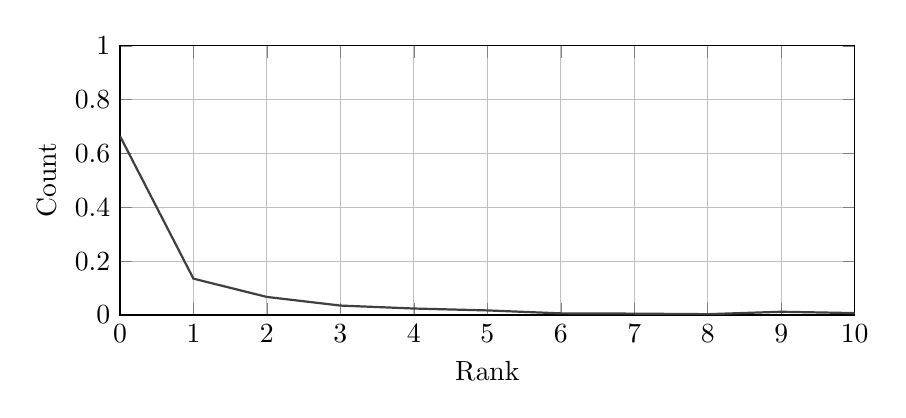
\begin{tikzpicture}[xscale=1,yscale=1]
\begin{axis}[xmin=0,xmax=10,ymin=0.0,ymax=1.00,no markers,grid=both,xlabel=Rank,ylabel=Count,width=0.9\textwidth,height=5cm]
\addplot[color=darkgray,thick] coordinates {(0, 0.665) (1, 0.135) (2, 0.067) (3, 0.035) (4, 0.024) (5, 0.017) (6, 0.006) (7, 0.005) (8, 0.003) (9, 0.012) (10, 0.007) (11, 0.006) (12, 0.003) (13, 0.004) (14, 0.002) (15, 0.0) (16, 0.002) (17, 0.002) (18, 0.0) (19, 0.0) (20, 0.0) (21, 0.001) (22, 0.002) (23, 0.0) (24, 0.0) (25, 0.0) (26, 0.0) (27, 0.0) (28, 0.0) (29, 0.0) (30, 0.0) (31, 0.0) (32, 0.0) (33, 0.0) (34, 0.001) (35, 0.0) (36, 0.0) (37, 0.0) (38, 0.0) (39, 0.0) (40, 0.0) (41, 0.0) (42, 0.0) (43, 0.0) (44, 0.0) (45, 0.0) (46, 0.0) (47, 0.0) (48, 0.0) (49, 0.0) (50, 0.001)};
\end{axis}
\end{tikzpicture}
\caption{Distribution of right key component ranks for 1000 experiments on $n=25$, $t=2.3$, $d=1$, $\mathrm{p}_{success}=0.99$.}
\label{fig:ranks}
\end{figure}

\anonymous{Our implementation will be made available soon.}{Our implementation is available at \url{http://bitbucket.org/malb/bkw-lwe}.}


}

\section{Parameters} \label{sec:parameters}
To understand the behaviour of our more careful modulus switching technique for concrete parameters, we compare it with one-shot modulus switching. Specifically, we consider the ``plain'' BKW algorithm \cite{blum-kalai-wasserman:acm2003} as analysed in \cite{albrecht-cid-faugere-fitzpatrick-perret:dcc2013}. Furthmore, to make this work somewhat self-contained we also compare with the BKZ (2.0) algorithm when applied to SIS instances derived from LWE samples and with a simple meet-in-the-middle (MITM) approach or generalised birthday attack.

\heading{Instances} We choose $n \in [128,256,512,1024,2048]$ and -- using \cite{albrecht-fitzpatrick-cabracas-goepfert-schneider:bitbucket2013} -- pick $q \approx n^2$ and $\sigma = \frac{q}{\sqrt{2\pi n} \log_2^2 n}$ as in Regev's original encryption scheme \cite{regev:acm09}. 
\submission{We then consider binary-LWE as defined in \cite{gentry-halevi-smart:crypto2012}: $\vec{s} \sample \U{\{-1,0,1\}^n}$ (we consider the case  $\vec{s} \sample \U{\Z_2^n}$ as in \cite{brakerski-langlois-peikert-regev-stehle:stoc13} in the full version of this work).}{We then consider both variants of what is known as binary-LWE in the literature: we first assume $\vec{s} \sample \U{\Z_2^n}$ as in \cite{brakerski-langlois-peikert-regev-stehle:stoc13} and then $\vec{s} \sample \U{\{-1,0,1\}^n}$ as in \cite{gentry-halevi-smart:crypto2012}.
}
However, we assume an unbounded number of samples being available to the attacker to establish the performance of the algorithms discussed here under optimal conditions.

\heading{BKW}
For complexity estimates of the plain BKW algorithm we rely on \cite{albrecht-cid-faugere-fitzpatrick-perret:dcc2013}. There the BKW algorithm takes a parameter $t$ which controls the addition depth $a := t \log_2 n$. Here we first pick $t = 2(\log_2 q - \log_2 \sigma)/\log_2 n$ which ensures that the standard deviation of the noise after $a$ levels of additions grows only as large as the modulus. We then slowly increase $t$ in steps of $0.1$ until the performance of the algorithm is not estimated to improve any further because too many samples are needed to perform the distinguishing step. Following \cite{albrecht-cid-faugere-fitzpatrick-perret:dcc2013}, we translate operations in $\Zq$ into ``bit operations'' by multiplying by $\log_2 q$.

\heading{BKZ}
To estimate the cost of the BKZ ($2.0$) algorithm we follow \cite{micciancio-regev:pqc2009,LindnerP10}. In \cite{micciancio-regev:pqc2009}, the authors briefly examine an approach for solving LWE by distinguishing between valid matrix-LWE samples of the form $(\mathbf{A},\mathbf{c})=(\mathbf{A},\mathbf{A}\vec{s}+\mathbf{e})$ and samples drawn from the uniform distribution over $\Zq^n\times\Zq$. Given a matrix of samples $\mathbf{A}$, one way of constructing such a distinguisher is to find a short vector $\mathbf{u}$ such that $\mathbf{u}\mathbf{A}=\mathbf{0}\bmod q$. If $\mathbf{c}$ belongs to the uniform distribution over $\Zq^n$, then $\langle\mathbf{u},\mathbf{c}\rangle$ belongs to the uniform distribution on $\Zq$. On the other hand, if $\mathbf{c}=\mathbf{A}\vec{s}+\mathbf{e}$, then $\langle\mathbf{u},\mathbf{c}\rangle=\langle\mathbf{u},\mathbf{A}\vec{s}+\mathbf{e}\rangle=\langle\mathbf{u},\mathbf{e}\rangle$, where samples of the form $\langle\mathbf{u},\mathbf{e}_i\rangle$ are governed by another discrete, wrapped Gaussian distribution. Following the work of Micciancio and Regev \cite{micciancio-regev:pqc2009}, the authors of \cite{LindnerP10} give estimates for the complexity of distinguishing between LWE samples and uniform samples by estimating the cost of the BKZ algorithm in finding a short enough vector. In particular, given $n, q, \sigma$ and a target distinguishing advantage $\epsilon$ we set $s = \sigma \cdot \sqrt{2\pi}$ and compute $\beta = q/s \cdot \sqrt{\log(1/\epsilon)/\pi}$. From this $\beta$ we then compute the required root Hermite factor $\delta_0 = 2^{ \log_2^2(\beta) / (4n\log_2 q ) }$. 

Given $\delta_0$ we then approximate the running time of BKZ 2.0 in seconds using two different strategies. Both strategies treat $\delta_0$ as the dominant influence in determining the running time.  The first strategy denoted ``BKZ'' follows \cite{LindnerP10} and defines $\log_2 T_{sec} = 1.8/\log_2 \delta_0 - 110$. The second strategy denoted ``BKZ2'' follows \cite{albrecht-cid-faugere-fitzpatrick-perret:dcc2013} who interpolated data points from \cite{liu-nguyen:ctrsa2013} as $\log_2 T_{sec} = 0.009/\log^2_2 \delta_0 - 27$.

We translate the running time in seconds figure into bit operations by assuming $2.3 \cdot 10^9$ bit operations per second on a 2.3~GHz CPU, which is pessimistic. Furthermore, for BKZ choosing advantage $\epsilon \ll 1$ and running the algorithms about $1/\epsilon$ times is usually more efficient than choosing $\epsilon \approx 1$ directly, i.e.\ we generate a new lattice of optimal sub-dimension each time using fresh LWE samples.

\heading{MITM} One can also solve small secret \LWE{} with a meet-in-the-middle attack that requires $\approx \mathfrak{c}^{n/2}$ time and space where $\mathfrak{c}$ is the cardinality of the set from which each component of the secret is sampled (so $\mathfrak{c}=2$ or $\mathfrak{c}=3$ for binary-LWE depending on the 
definition used): compute and store a sorted list of all $\vec{A}\vec{s'}$ where $\vec{s'} = (\vec{s}_{(0)},\dots, \vec{s}_{(n/2)-1}, 0, 0, \ldots, 0)$ 
for all possible $\mathfrak{c}^{n/2}$ choices for $\vec{s'}$. Then compute $\vec{c} - \vec{A}\vec{s''}$ where we have $\vec{s''} = (0, 0, \ldots, 0,\vec{s}_{(n/2)},\ldots, \vec{s}_{n-1})$ and check for a vector that is close to this value in the list.

\submission{}{
\heading{Results for $\vec{s} \sample \U{\Z_2^n}$}
In Table~\ref{tab:nomodred} we give the number of bit operations (``$\log \Z_2$''), calls to the LWE oracle (``$\log \Ldis$'') and memory requirement (``$\log \textnormal{mem}$'') for BKW without any modulus reduction to establish the baseline. All costs are given for the high advantage case, i.e.\ if $\epsilon\ll 1$ we multiply the cost by $1/\epsilon$.
\begin{table}
\centering\ifthenelse{\equal{\isshort}{1}}{\scriptsize}{}
\begin{tabular}{|r||r|r||r|r|r||r|r|r||r|r|r|r|}
\hline
   & \multicolumn{2}{|c||}{MITM}& \multicolumn{3}{|c||}{BKZ \cite{LindnerP10}} & \multicolumn{3}{|c||}{BKZ $2.0$ \cite{liu-nguyen:ctrsa2013}} & \multicolumn{4}{|c|}{BKW \cite{albrecht-cid-faugere-fitzpatrick-perret:dcc2013}}\\
\hline
$n$ & $\log \Z_2$ & $\log \textnormal{mem}$ & $\log \epsilon$ & $\log \Ldis$ & $\log \Z_2$ & $\log \epsilon$ & $\log \Ldis$ & $\log \Z_2$ & $t$ &  $\log \Ldis$ & $\log \Z_2$ & $\log \textnormal{mem}$\\
\hline
%  32 &   16 &   16 &     -8 &     14.4 &    -30.5 &     -3 &      9.5 &     13.8 &  3.39 &     28.5 &     40.0 &     26.2 \\
%  64 &   32 &   32 &    -12 &     19.4 &      3.4 &     -6 &     13.5 &     27.4 &  3.17 &     43.7 &     55.9 &     48.8 \\
 128 &   67.8 &   64 &    -18 &     26.5 &     65.4 &    -14 &     22.5 &     65.7 &  3.18 &     83.9 &     97.6 &     90.0 \\
 256 &  132.0 &  128 &    -29 &     38.5 &    179.5 &    -35 &     44.5 &    178.5 &  3.13 &    167.2 &    182.1 &    174.2 \\
 512 &  260.2 &  256 &    -48 &     58.5 &    390.9 &    -94 &    104.5 &    522.8 &  3.00 &    344.7 &    361.0 &    352.8 \\
1024 &  516.3 &  512 &    -82 &     93.5 &    785.0 &   -265 &    276.5 &   1606.2 &  2.99 &    688.0 &    705.5 &    697.0 \\
2048 & 1028.5 & 1024 &   -141 &    153.6 &   1523.6 &   -773 &    785.4 &   5100.0 &  3.00 &   1369.8 &   1388.7 &   1379.9 \\
\hline
\end{tabular}
\caption{Cost for solving Decision-\LWE with advantage $\approx 1$ for BKW, BKZ and MITM where $q,\sigma$ are chosen as in \cite{regev:acm09} and $\vec{s} \sample \U{\Z_2^n}$. We run BKZ $1/\epsilon$ times, ``$\log \Z_2$'' gives the number of ``bit operations'', ``$\log \Ldis$'' the number of \LWE oracle calls 
and ``$\log \textnormal{mem}$'' the memory requirement of $\Zq$ elements. All logarithms are base $2$.}
\label{tab:nomodred}
\end{table}
Table~\ref{tab:modred} gives the running times after modulus reduction with $p = q\sqrt{n/12}\sigma_s/\sigma$. In particular, Table~\ref{tab:modred} lists the expected running time (number of oracle calls and where applicable memory requirements) of running BKW and BKZ after applying modulus reduction.

\begin{table}
\centering\ifthenelse{\equal{\isshort}{1}}{\scriptsize}{}
\begin{tabular}{|r||r|r|r||r|r|r||r|r|r|r|}
\hline
    & \multicolumn{3}{|c||}{BKZ \cite{LindnerP10}} & \multicolumn{3}{|c||}{BKZ $2.0$ \cite{liu-nguyen:ctrsa2013}} & \multicolumn{4}{|c|}{BKW \cite{albrecht-cid-faugere-fitzpatrick-perret:dcc2013}}\\
\hline
$n$ & $\log \epsilon$ & $\log \Ldis$ & $\log \Z_2$ & $\log \epsilon$ & $\log \Ldis$ & $\log \Z_2$ & $t$ &  $\log \Ldis$ & $\log \Z_2$ & $\log \textnormal{mem}$\\
\hline
%  32 &    -11 &     17.4 &    -21.6 &     -5 &     11.5 &     17.8 &  2.82 &     28.5 &     39.4 &     25.5 \\
%  64 &    -14 &     21.3 &     10.6 &     -8 &     15.4 &     31.7 &  2.73 &     40.9 &     52.5 &     46.0 \\
 128 &    -20 &     28.3 &     68.5 &    -16 &     24.3 &     68.6 &  2.84 &     76.1 &     89.6 &     81.2 \\
 256 &    -31 &     40.3 &    172.5 &    -36 &     45.3 &    169.5 &  2.74 &    149.6 &    164.0 &    156.7 \\
 512 &    -49 &     59.3 &    360.2 &    -89 &     99.2 &    457.8 &  2.76 &    289.8 &    305.6 &    297.9 \\
1024 &    -80 &     91.3 &    701.6 &   -232 &    243.2 &   1312.8 &  2.78 &    563.1 &    580.2 &    572.2 \\
2048 &   -133 &    145.3 &   1327.6 &   -636 &    648.1 &   3929.5 &  2.71 &   1135.3 &   1153.6 &   1145.3 \\
\hline
\end{tabular}
\caption{Cost for solving Decision-LWE with advantage $\approx 1$ for BKW and BKZ variants where $q,\sigma$ are chosen as in \cite{regev:acm09} and $\vec{s} \sample \U{\Z_2^n}$ after one-shot modulus reduction with $p = q\sqrt{n/12}\sigma_s/\sigma$.}
\label{tab:modred}
\end{table}

Finally, Table~\ref{tab:thiswork} gives the expected costs for solving these \LWE{} instances using the techniques described in this work. We list two variants: one with and one without ``unnatural selection'' . This is because these techniques rely on more assumptions than the rest of this work which means we have greater confidence in the predictions avoiding such assumptions. Yet, as discussed in Section~\ref{sec:implementation}, these assumptions seem to hold reasonably well in practice.

\begin{table}
\centering\ifthenelse{\equal{\isshort}{1}}{\scriptsize}{}
\begin{tabular}{|r||r|r|r|r|r|r||r|r|r|r|r|r|r|r|}
\hline
   & \multicolumn{6}{|c||}{this work (w/o unnatural selection)} & \multicolumn{6}{|c|}{this work}\\
\hline
$n$ & $t$ & $\log p$ & $\log m^\ast$ & $\log \Ldis$ & $\log \Z_2$ & $\log \textnormal{mem}$ & $t$ & $\log p$ & $\log m^\ast$ & $\log \Ldis$ & $\log \Z_2$ & $\log \textnormal{mem}$\\
\hline
%  32 &  3.39 & 10 &    0 &     28.5 &     40.0 &     26.1  & 3.39 & 10 &    0 &     28.5 &     40.0 &     26.1\\ %     28.5
%  64 &  3.17 & 10 &    0 &     37.0 &     49.2 &     42.1  & 3.17 &  7 &   34 &     34.8 &     47.6 &     32.0\\ %     33.5
 128 &  2.98 & 10 &    0 &     64.7 &     78.2 &     70.8  & 2.98 &  6 &   60 &     60.0 &     74.2 &     46.3\\ %     39.7
 256 &  2.83 & 11 &    0 &    127.8 &    142.7 &    134.9  & 2.83 &  5 &  117 &    117.0 &    132.5 &     67.1\\ %     41.2
 512 &  2.70 & 11 &    0 &    235.1 &    251.2 &    243.1  & 2.70 &  8 &  225 &    225.0 &    241.8 &    180.0\\ %     31.8
1024 &  2.59 & 12 &    0 &    477.4 &    494.8 &    486.5  & 2.59 & 10 &  467 &    467.0 &    485.0 &    407.5\\ %     29.9
2048 &  2.50 & 12 &    0 &    897.8 &    916.4 &    907.9  & 2.50 & 10 &  834 &    834.0 &    853.2 &    758.9\\ %     36.4
\hline
\end{tabular}
\caption{Cost for solving Decision-\LWE{} with advantage $\approx 1$ with the algorithms discussed in this work when $\vec{s} \sample \U{\Z_2^n}$.}
\label{tab:thiswork}
\end{table}
}

\submission{In Table~\ref{tab:nomodred2} we give the number of bit operations (``$\log \Z_2$''), calls to the LWE oracle (``$\log \Ldis$'') and memory requirement (``$\log \textnormal{mem}$'') for BKW without any modulus reduction to establish the baseline. All costs are given for the high advantage case, i.e.\ if $\epsilon\ll 1$ we multiply the cost by $1/\epsilon$.
}{\heading{Results for $\vec{s} \sample \U{\{-1,0,1\}^n}$} Tables~\ref{tab:nomodred2}, \ref{tab:modred2} and \ref{tab:thiswork2} correspond to Tables~\ref{tab:nomodred}, \ref{tab:modred} and \ref{tab:thiswork} and adopt the same notation.}

\begin{table}
\centering\ifthenelse{\equal{\isshort}{1}}{\scriptsize}{}
{
\begin{tabular}{|r||r|r||r|r|r||r|r|r||r|r|r|r|}
\hline
   & \multicolumn{2}{|c||}{MITM}& \multicolumn{3}{|c||}{BKZ \cite{LindnerP10}} & \multicolumn{3}{|c||}{BKZ $2.0$ \cite{liu-nguyen:ctrsa2013}} & \multicolumn{4}{|c|}{BKW \cite{albrecht-cid-faugere-fitzpatrick-perret:dcc2013}}\\
\hline
$n$ & $\log \Z_2$ & $\log \textnormal{mem}$ & $\log \epsilon$ & $\log \Ldis$ & $\log \Z_2$ & $\log \epsilon$ & $\log \Ldis$ & $\log \Z_2$ & $t$ &  $\log \Ldis$ & $\log \Z_2$ & $\log \textnormal{mem}$\\
\hline
%  32 &   25.4 &   25.4 &     -8 &     14.4 &    -30.5 &     -3 &      9.5 &     13.8 &  3.39 &     28.5 &     40.0 &     26.2 \\
%  64 &   50.7 &   50.7 &    -12 &     19.4 &      3.4 &     -6 &     13.5 &     27.4 &  3.17 &     43.7 &     55.9 &     48.8 \\
  128 &  105.2 &  101.4 &    -18 &     26.5 &     65.4 &    -14 &     22.5 &     65.7 &  3.18 &     83.9 &     97.6 &     90.0 \\
  256 &  206.9 &  202.9 &    -29 &     38.5 &    179.5 &    -35 &     44.5 &    178.5 &  3.13 &    167.2 &    182.1 &    174.2 \\
  512 &  409.9 &  405.8 &    -48 &     58.5 &    390.9 &    -94 &    104.5 &    522.8 &  3.00 &    344.7 &    361.0 &    352.8 \\
 1024 &  815.8 &  811.5 &    -82 &     93.5 &    785.0 &   -265 &    276.5 &   1606.2 &  2.99 &    688.0 &    705.5 &    697.0 \\
 2048 & 1627.5 & 1623.0 &   -141 &    153.6 &   1523.6 &   -773 &    785.4 &   5100.0 &  3.00 &   1369.8 &   1388.7 &   1379.9 \\
\hline
\end{tabular}
}
\caption{Cost for solving Decision-LWE with advantage $\approx 1$ for BKW, BKZ and MITM where $q$ and $\sigma$ are chosen as in \cite{regev:acm09} and 
$\vec{s} \sample \U{\{-1,0,1\}^{n}}$.}
\label{tab:nomodred2}
\end{table}

\submission{Table~\ref{tab:modred2} gives the running times after modulus reduction with $p = q\sqrt{n/12}\sigma_s/\sigma$. In particular, Table~\ref{tab:modred2} lists the expected running time (number of oracle calls and where applicable memory requirements) of running BKW and BKZ after applying modulus reduction.}

\begin{table}
\centering\ifthenelse{\equal{\isshort}{1}}{\scriptsize}{}
\begin{tabular}{|r||r|r|r||r|r|r||r|r|r|r|}
\hline
    & \multicolumn{3}{|c||}{BKZ \cite{LindnerP10}} & \multicolumn{3}{|c||}{BKZ $2.0$ \cite{liu-nguyen:ctrsa2013}} & \multicolumn{4}{|c|}{BKW \cite{albrecht-cid-faugere-fitzpatrick-perret:dcc2013}}\\
\hline
$n$ & $\log \epsilon$ & $\log \Ldis$ & $\log \Z_2$ & $\log \epsilon$ & $\log \Ldis$ & $\log \Z_2$ & $t$ &  $\log \Ldis$ & $\log \Z_2$ & $\log \textnormal{mem}$\\
\hline
%  32 &    -11 &     17.4 &    -21.3 &     -5 &     11.5 &     17.9 &  2.85 &     28.5 &     39.5 &     25.8 \\
%  64 &    -14 &     21.4 &     11.6 &     -8 &     15.4 &     32.2 &  2.74 &     41.5 &     53.2 &     46.6 \\
  128 &    -21 &     29.3 &     70.2 &    -16 &     24.4 &     69.8 &  2.85 &     76.8 &     90.2 &     82.4 \\
  256 &    -31 &     40.3 &    175.3 &    -37 &     46.3 &    172.8 &  2.85 &    150.4 &    165.6 &    153.7 \\
  512 &    -50 &     60.3 &    365.0 &    -90 &    100.2 &    467.0 &  2.76 &    293.8 &    309.6 &    301.9 \\
 1024 &    -81 &     92.3 &    710.1 &   -236 &    247.2 &   1339.1 &  2.78 &    570.3 &    587.4 &    579.4 \\
 2048 &   -134 &    146.3 &   1342.3 &   -647 &    659.2 &   4006.5 &  2.71 &   1149.0 &   1167.3 &   1159.1 \\
\hline
\end{tabular}
\caption{Cost for solving Decision-LWE with advantage $\approx 1$ for BKW and BKZ variants where $q,\sigma$ are chosen as in \cite{regev:acm09} and 
$\vec{s} \sample \U{\{-1,0,1\}^n}$ after one-shot modulus reduction with $p = q\sqrt{n/12}\sigma_s/\sigma$.}
\label{tab:modred2}
\end{table}

\submission{Finally, Table~\ref{tab:thiswork2} gives the expected costs for solving these \LWE instances using the techniques described in this work. We list two variants: one with and one without ``unnatural selection''. This is because these techniques rely on more assumptions than the rest of this work which means we have greater confidence in the predictions avoiding such assumptions.}{}

\begin{table}
\centering\ifthenelse{\equal{\isshort}{1}}{\scriptsize}{}
\begin{tabular}{|r||r|r|r|r|r|r||r|r|r|r|r|r|r|r|}
\hline
   & \multicolumn{6}{|c||}{this work (w/o unnatural selection)} & \multicolumn{6}{|c|}{this work}\\
\hline
$n$ & $t$ & $\log p$ & $\log m^\ast$ & $\log \Ldis$ & $\log \Z_2$ & $\log \textnormal{mem}$ & $t$ & $\log p$ & $\log m^\ast$ & $\log \Ldis$ & $\log \Z_2$ & $\log \textnormal{mem}$ \\
\hline
%  32 &  3.39 & 10 &    0 &     28.5 &     40.0 &     26.1 & 3.39 & 10 &    0 &     28.5 &     40.0 &     26.1\\ %     28.5 
%  64 &  3.17 & 10 &    0 &     37.0 &     49.2 &     42.1 & 3.17 &  7 &   35 &     35.3 &     48.2 &     32.0\\ %     33.0 
  128 &  2.98 & 10 &    0 &     64.7 &     78.2 &     70.8 & 2.98 &  6 &   61 &     61.0 &     75.2 &     46.3\\ %     40.9 
  256 &  2.83 & 11 &    0 &    127.8 &    142.7 &    134.9 & 2.83 &  5 &  118 &    118.0 &    133.5 &     67.1 \\ %     44.3 
  512 &  2.70 & 11 &    0 &    235.1 &    251.2 &    243.1 & 2.70 &  8 &  225 &    225.0 &    241.8 &    180.0 \\ %     32.9 
 1024 &  2.59 & 12 &    0 &    477.4 &    494.8 &    486.5 & 2.59 & 10 &  467 &    467.0 &    485.0 &    407.5 \\ %     30.4 
 2048 &  2.50 & 12 &    0 &    971.4 &    990.7 &    907.9 & 2.50 & 12 &  961 &    961.0 &    980.2 &    907.9 \\ %     30.9 
\hline
\end{tabular}
\caption{Cost for solving Decision-LWE with advantage $\approx 1$ with the algorithms discussed in this work when $\vec{s} \sample \U{\{-1,0,1\}^n}$.}
\label{tab:thiswork2}
\end{table}

\heading{Discussion}
The results in this section\submission{}{ (summarised in Figure~\ref{fig:plot-c2})} indicate that the variants of the BKW algorithms discussed in this work compare favourably for the paramters considered. \submission{}{In particular, in the case $\vec{s} \sample \U{\{0,1\}^n}$ these BKW variants are the only algorithms which beat the simple MITM approach. For $\vec{s} \sample \U{\{-1,0,1\}^n}$ that advantage naturally increases.} The results in this table also indicate that the unnatural selection strategy has little impact on the overall time complexity. However, it allows to reduce the data complexity, in some cases, considerably. In particular, e.g.\ considering line 1 of Table~\ref{tab:thiswork2}, we note that applying this technique can make the difference between a feasible ($\approx 80 \cdot 1024^4$ bytes) and infeasible ($\approx 1260 \cdot 1024^6$ bytes) attack for a well-equipped attacker \cite{utah-data-centre}. Finally, we note that our results indicate that lattice reduction benefits from modulus reduction. However, this seems somewhat implausible judging from the used algorithms. This might indicate that the lattice reduction estimates from the literature  above might need to be revised.

\submission{}{
\begin{figure}
\centering
\begin{tabular}{c}
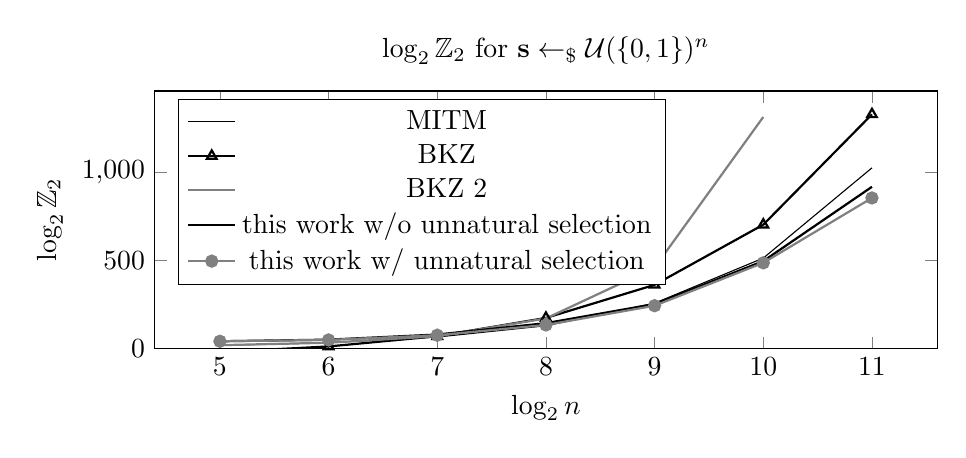
\begin{tikzpicture}
\ifthenelse{\equal{\isshort}{1}}
{\pgfplotsset{width=.95\textwidth, height=0.3\textwidth}}
{\pgfplotsset{width=.95\textwidth, height=0.4\textwidth}}
\begin{axis}[xlabel={$\log_2 n$},ylabel={$\log_2 \Z_2$},ymin=0,legend pos=north west,title={$\log_2 \Z_2$ for $\vec{s} \sample \U{\{0,1\}}^n$}]
\addplot[black] coordinates {( 5,   16) ( 6,   32) ( 7,  64) ( 8,  128) ( 9,  256) (10,  512) (11, 1024) };
\addlegendentry{MITM};

\addplot[black,thick,mark=triangle] coordinates { (5, -21.60)  (6, 10.60)  (7, 68.50)  (8, 172.50)  (9, 360.20)  (10, 701.60)  (11, 1327.60) };
\addlegendentry{BKZ};

\addplot[gray,thick] coordinates { (5, 17.80)  (6, 31.70)  (7, 68.60)  (8, 169.50)  (9, 457.80)  (10, 1312.80) };
\addlegendentry{BKZ 2};

\addplot[black,thick,mark=circle] coordinates { (5, 40.00)  (6, 49.20)  (7, 78.20)  (8, 142.70)  (9, 251.20)  (10, 494.80)  (11, 916.40) };
\addlegendentry{this work w/o unnatural selection};

\addplot[gray,thick,mark=*] coordinates { (5, 40.00)  (6, 47.60)  (7, 74.20)  (8, 132.50)  (9, 241.80)  (10, 485.00)  (11, 853.20)};
\addlegendentry{this work w/ unnatural selection};
\end{axis}\end{tikzpicture}
\\
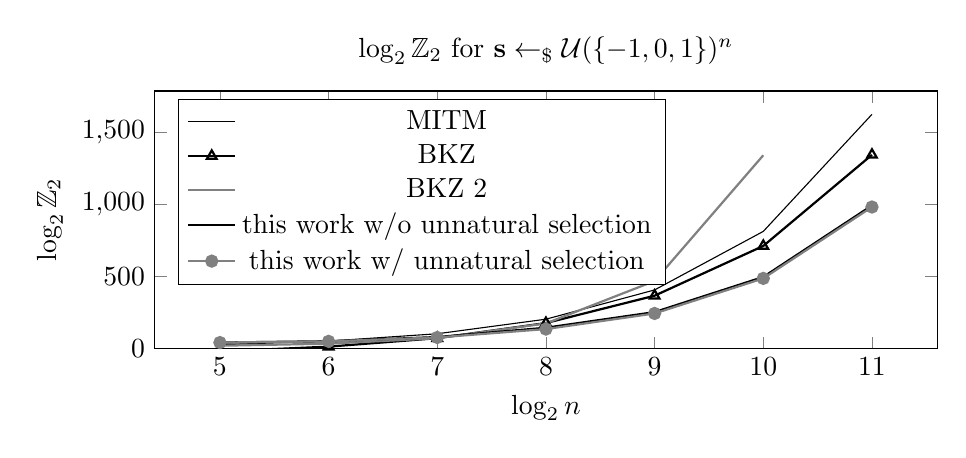
\begin{tikzpicture}
\ifthenelse{\equal{\isshort}{1}}
{\pgfplotsset{width=.95\textwidth, height=0.3\textwidth}}
{\pgfplotsset{width=.95\textwidth, height=0.4\textwidth}}
\begin{axis}[xlabel={$\log_2 n$},ylabel={$\log_2 \Z_2$},ymin=0,legend pos=north west,title={$\log_2 \Z_2$ for $\vec{s} \sample \U{\{-1,0,1\}}^n$}]
\addplot[black] coordinates { (5, 25.00)  (6, 50.00)  (7, 101.00)  (8, 202.00)  (9, 405.00)  (10, 811.00)  (11, 1623.00) };
\addlegendentry{MITM};

\addplot[black,thick,mark=triangle] coordinates { (5, -21.30)  (6, 11.60)  (7, 70.20)  (8, 175.30)  (9, 365.00)  (10, 710.10)  (11, 1342.30)  };
\addlegendentry{BKZ};

\addplot[gray,thick] coordinates { (5, 17.90)  (6, 32.20)  (7, 69.80)  (8, 172.80)  (9, 467.00)  (10, 1339.10)  };
\addlegendentry{BKZ 2};

\addplot[black,thick,mark=circle] coordinates { (5, 40.00)  (6, 49.20)  (7, 78.20)  (8, 142.70)  (9, 251.20)  (10, 494.80)  (11, 990.70)  };
\addlegendentry{this work w/o unnatural selection};

\addplot[gray,thick,mark=*] coordinates { (5, 40.00)  (6, 48.20)  (7, 75.20)  (8, 133.50)  (9, 241.80)  (10, 485.00)  (11, 980.20) };
\addlegendentry{this work w/ unnatural selection};
\end{axis}
\end{tikzpicture}
\end{tabular}
\label{fig:plot-c2}
\caption{Cost of solving Decision-\LWE{} using various algorithms discussed in this work.}
\end{figure}
}

\submission{}{
\heading{Reproducibility} Since the results of this section rely on estimates which involve numerical approximations we make the source code (written for Sage~\cite{sagemath}) we used to compute these figures available as an attachment to this document. \embedfile{bkw-small-secret.py}}

\section{Conclusion \& Future Work}

We investigated applying modulus switching to exploit the presence of a small secret in LWE instances and demonstrated that it can make a significant impact on the complexity of solving such instances. We also adapted the BKW algorithm to perform modulus-switching `on-the-fly', showing that this approach is superior to performing `one-shot' modulus reduction on LWE samples prior to solving. Our first variant improves the target modulus by a factor of $\sqrt{\log_2 n}$ in typical scenarios; our second variant mainly improves the memory requirements of the algorithm, one of the key limiting aspects of the BKW algorithm. Our algorithms, however, rely on various assumptions which, though appearing sound, are unproven. Our estimates should thus be considered heuristic, as are performance estimates for all currently-known algorithms for solving LWE. Verifying these assumptions is hence a promising direction for future research. Furthermore, one of the main remaining obstacles for applying the BKW algorithm to cryptographic constructions based on LWE is that it requires an unbounded number of samples to proceed. Lifting this requirement, if only heuristically, is hence a pressing research question.

\section*{Acknowledgement}
We thank Steven Galbraith for helpful comments on an earlier draft of this work. We also thank anonymous referees for detailed comments which greatly improved this work. Jean-Charles Faugère, and Ludovic Perret  have been partially supported supported by the Computer Algebra and Cryptography (CAC) project (ANR-09-JCJCJ-0064-01) and the HPAC grant (ANR ANR-11-BS02-013) of the French National Research Agency. 

\bibliographystyle{plain}
\bibliography{bkw-small-secret}

\end{document}
